\chapter{Tyranid Acquisition}

\begin{wrapfigure}{O}{\figwidth}
	\begin{center}
		
\includegraphics[width=\figwidth]{pics/12/1.png}
	\end{center}
\end{wrapfigure}
Interrogator Greg Sargent stood with his group of experts and contemplated the door. 
It was larger and fancier than any of the others in the hallway, and it was also the only door that had been welded shut. 
The words "Psyker Holding Cells" could just barely be seen under the swathes of prayer seals that covered the door. 
Sarge shuddered at the memories those words dredged up and silently cursed whoever had decided to leave the damned section in during the ship's refit.

At a wave from Sarge, Chief Engineer Ol' Bill and Senior Enginseer Jim moved forwards. 
They ignored the official little yellow plaque which promised a slow and painful death for anyone who opened the door, and began cutting. 
At the back of the group, Senior Enginseer Hannah and the ship's Confessor explained why the door had been sealed to a worried looking Xenologist Adept. 
When the Xenologist started backing away and suggesting that he really didn't need to personally inspect the Cells, Sarge cut in and assured him that the daemon which had haunted the place was very thoroughly dead.

Once the door was cut open, the Confessor led the way inside with a censer in one hand and a flamer filled with holy promethium in the other. 
Sarge thought the priest seemed disappointed when nothing jumped out and tried to eat his soul. 
The Confessor gave the all-clear and the whole group trooped in and started assessing the Cells.

The main room was circular, filled with several pieces of arcane machinery, and was connected via very-thick doors to a dozen child-sized holding cells. 
Eleven of those cells were open and looked exactly the same as when Sarge had last seen them, the twelfth didn't. 
Instead of the ominously locked door he'd remembered, it was a jagged crater partially filled with debris from it's half-collapsed ceiling. 
The delicate machinery immediately around the crater had been turned to scrap by door-shrapnel, and a few clawed foot-prints could be seen in the wreckage.

\begin{wrapfigure}{O}{\figwidth}
	\begin{center}
		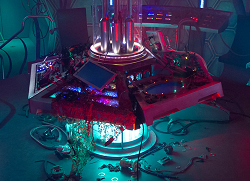
\includegraphics[width=\figwidth]{pics/12/2.png}
	\end{center}
\end{wrapfigure}
One by one, the technical experts reported their findings to the Xenologist Adept. 


Ol' Bill reported that the Warp-Presence Shroud was missing a certain key component and would be barely functional. 
The Xenologist asked if "missing" meant it might be found somewhere, and Sarge explained that in this case it meant that the piece was welded into the warp-drive. 
Ol' Bill recommended leaving that part where it was.

Jim followed that up with the news that the Cells' Psi-Suppressor had been badly damaged, but he was reasonably confident that by cannibalizing parts and reducing coverage it could be gotten back up to eighty percent power. 
Jim refused to guess whether that was Delta, Epsilon, or a lower level psi-suppression, citing his own lack of any idea how the damned thing worked. 
The Xenologist winced at hearing this.

Finally Hannah reported that all eleven intact stasis units were in working order. 
The problem was that, unless the specimen was going to be child-sized, there'd be no way to fit it in one. 
Putting it half-inside a stasis field would result in a half-specimen, trying to overlap the fields would result in a rather large explosion, and there was no Mechanicus-approved method for kludging multiple stasis units into a larger one. 
When the Xenologist claimed that there was no way anything would work without a stasis-field, Hannah grudgingly admitted that Tink and his "assistant" might have some not-entirely-orthodox way of doing it. 
Sarge groaned at that, but didn't actually say anything.

Everyone went quiet as the Adept digested the lackluster reports. 
In the silence Sarge noticed a faint sound coming from the debris-clogged cell. 
A laspistol practically materialized in his hands, and he motioned everyone except the well-armed Confessor back.

\begin{wrapfigure}{O}{\figwidth}
	\begin{center}
		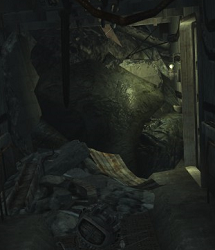
\includegraphics[width=\figwidth]{pics/12/3.png}
	\end{center}
\end{wrapfigure}
As the two men carefully pushed aside pieces of wreckage, the sound grew clearer. 
It was a sort of far-off chattering, screaming sound, mixed with what sounded like the thump of heavy crates being moved around, and a familiar nasal voice talking to itself.

Everyone in the room groaned, except for Sarge, who thrust his head as far as he could into the wrecked cell and bellowed "GODDAMNIT NUBBY."

There was an inarticulate scream and the sound of several objects falling over. 
When the clattering died away a plaintive "Bloody 'ell Sarge, chu doin down 'ere?" drifted out from somewhere in the rear of the cell.

Sarge began ripping out pieces of wreckage in an effort to find where the trooper was hiding. 
As he worked the enraged noncom embarked on what was sure to be an epic chewing-out. 
"What am I doing? 
WHAT AM I DOING? 
What are YOU doing you little idiot? 
And why in the Emperor's name are you doing it in the Psyker Holding Cells?"

Nubby's tone grew panicked as he registered Sarge's fury. 
"I aint doin nufin! 
An' you made me promise na ta go nowhere near yer stupid cells. 
I'm jus' mindin me own business down at da bottom of da liffs."

This gave Sarge pause, and in the silence the faint chattering screaming he'd been hearing under Nubby's voice finally registered. 
Sarge groaned as the realization hit him. 
The Confessor, who didn't know Nubby quite as well, asked if he was in the Chapel to the Emperor located in the deck below the lift to the bridge. 
Nubby's hesitant reply of "sorta" was cut off by Sarge. 


"Nubby are you using the containment area inside the Chapel, the one we built around the unholy screaming crater the Cogtain left when he died, to store contraband?"

"... 
no?"

"Really Nubby?"

"Well, not really contraband per se, jus' like, odds an' ends."

"GODDAMN IT NUBBY!"

"It's not like anyone was usin it!"

\begin{wrapfigure}{O}{\figwidth}
	\begin{center}
		
\includegraphics[width=\figwidth]{pics/12/4.png}
	\end{center}
\end{wrapfigure}
While Sarge and the Confessor both sputtered in a mix of horror and frustration, Jim raised the question of how the conversation was actually happening. 
Sarge couldn't see anything through the gaps in the debris besides the cell's rear wall. 
He grudgingly ordered Nubby to search the containment room for any sort of communicator or portal.

Nubby followed their voices, and reported the glowing crater left by the dead Cogtain as the source. 
He hesitantly asked if glowing metal could be a portal, and if he should try poking it with something.

Sarge's answer was drowned out by a screeching flood of daemonic and binary screaming. 
The noise rose a crescendo as the far wall of the cell started glowing and a jagged length of metal poked through. 
The blade flailed around like a snake stuck in a hole, and slowly hauled something that looked like a cross between a lasgun's barrel and a daemonic skull out behind it. 
Sarge leapt aside as the Confessor ran forwards and hosed the back of the cell with sanctified promethium.

When the noise finally died down, Nubby's voice returned and asked if anyone had seen where his lasgun had gone after the metal ate it. 
Sarge told him it was probably time to get a new gun from Tink, and ordered the trooper to return to his quarters immediately. 
Without any of his "odds an' ends."

As the faint sound of Nubby's metal footsteps and curses faded away, Sarge turned to where the Xenologist was trying to hide behind Ol' Bill.
\begin{wrapfigure}{O}{\figwidth}
	\begin{center}
		
\includegraphics[width=\figwidth]{pics/12/5.png}
	\end{center}
\end{wrapfigure}
"Right... 
we'll worry about that later, back to why we're actually down here. 
You've heard the reports, do you think we can do it?"

"Okay, just to be clear."

"Yes."

"We have a Psyker Containment Area with almost no warp-presence shrouding, an indeterminate amount of psi-suppression, and a stasis field that'll be kludged together from smaller units by that mad xenos you've got hiding in your quarters."

"Uh-huh."

"And you're asking if we can use this Area, which is already so tainted that it's manifesting major phenomena, to hold a live Tyranid Zoanthrope for a months-long warp voyage?"

"That's right."

"That is quite literally the worst idea I've ever heard."

\greentext{>The All Guardsmen Party: Tyranid Acquisition Experts}


\begin{wrapfigure}{O}{\figwidth}
	\begin{center}
		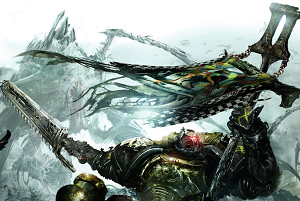
\includegraphics[width=\figwidth]{pics/12/6.png}
	\end{center}
\end{wrapfigure}
So no shit, there we were, heading out beyond the fringes of Imperial Space to capture a xenos psyker, which we would then have to haul, kicking and screaming, half-way across the galaxy. 
There were probably shitier missions out there, but that wasn't much comfort. 
Saying "It could always be worse" loses it's charm when things actually DO keep getting worse. 


The only thing that kept us from labeling it as a suicide mission was the fact that a force from the Emperor's Scythes Space Marine chapter would be leading the actual capture effort. 
In fact it was technically their mission, we were just supposed to assist them in the capture, then handle the transport. 
The fact that we'd be working with, and fighting alongside, a team of Space Marines didn't actually make us much happier though. 


I mean sure, the Marines are the greatest warriors in all the Imperium, near-immortal demigods of war and all that, but we'd been in our share of battles. 
Every one of us had seen what inevitably happens when the Astartes get called in: 
the quickest way for a Guardsman to meet the Emperor is to be anywhere within a ten-kilometer radius of one of His angels.

Sadly, the assignment had come directly from Inquisitor Oak, so there was nothing we could do to avoid it. 
No matter how insane the mission, how bad our equipment, and how certain our deaths, there was nothing short of desertion that would get us out of our orders. 
So we went to work preparing our equipment and took solace in the most sacred right of all soldiers: 
complaining.

\begin{wrapfigure}{O}{\figwidth}
	\begin{center}
		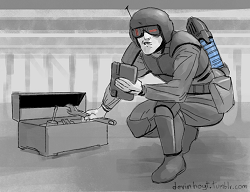
\includegraphics[width=\figwidth]{pics/12/7.png}
	\end{center}
\end{wrapfigure}
To start with, Tink complained about how unfair it was to stick him and Fio, our semi-captive Tau scientist, with so much to do in so little time. 
The two of them worked furiously on the problem of combining the smaller stasis units into a larger one, while simultaneously trying to cram more pulse weapons into lasgun disguises and build Spot 2.0. 
Their efforts were seriously hampered by the fact that Tau science isn't anywhere near as advanced when it comes to stasis fields, or anything related to psykers for that matter, as it is on the subject of plasma or drones. 
Then, on top of that, there was the whole heretical xenotech on an Imperial vessel issue.

The xenotech problem wasn't as serious as it used to be: 
replacing all of our annoying old cogboys with slightly-less-annoying young cogboys had resulted in far more liberal outlook among the ship's tech-priesthood. 
Sarge still insisted on a moderate amount of discretion though, which caused significant slowdowns, especially when combined with Jim's newfound stodginess as head-cogboy. 


Mister I'm-a-big-boy-now Head Enginseer Jim flat-out insisted that none of the junior tech-priests were allowed to even work in the same room as Fio, much less lend a mechadendrite. 
We sort of understood that it was all for the safety of the acolytes, who might get in deep trouble if they displayed bad habits in their future postings, but it slowed things down considerably. 
Tink wound up drafting Sarge and most of the adepts as assistants; 
none of them were very helpful mind you, but the fact that they were suffering with him cheered Tink up immensely.
\begin{wrapfigure}{O}{\figwidth}
	\begin{center}
		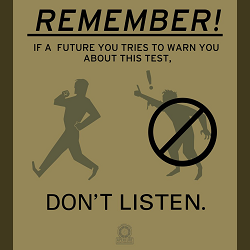
\includegraphics[width=\figwidth]{pics/12/8.png}
	\end{center}
\end{wrapfigure}
Jim, Hannah, and Ol' Bill did their fair share of complaining too. 
The projects they were working on weren't much easier than Tink's, and they also were trying to keep the ship running and train their new recruits. 
In the long run the fresh batch of cogboys was probably going to work out wonderfully, but in the short term it was complete mayhem. 
Hannah had it especially bad, since she was the one in charge of the newbies while the others ran their projects. 
She was driven to the edge of hysterics by a constant barrage of questions and problems, ranging from trivial to potentially fatal, from the Acolytes. 
The poor cog-girl hid from them in our barracks more than once.

While the technical folks whined about over-work, Doc, Fumbles, and the Xenologist Adept complained to anyone who would listen about being used as human guinea pigs. 
Really, all of them understood there were no other options for testers, and the Containment Area had to be tested. 
They just hated the fact that said testing consisted of the Xenologist coaxing Fumbles into trying to manifest the sort of powers a Zoanthrope might use, while Doc stood around and waited to fix whatever went wrong. 
And when you combine Fumbles trying to use powers outside his comfort zone, a high-stress environment, and the quality the Containment Area, you better believe things went wrong. 
At least Doc did got a lot of practice fixing up injured cogboys, so there was some silver lining.
\begin{wrapfigure}{O}{\figwidth}
	\begin{center}
		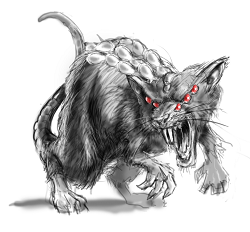
\includegraphics[width=\figwidth]{pics/12/9.png}
	\end{center}
\end{wrapfigure}
The only members of the team who weren't involved in preparing the Containment Area were Nubby, Twitch, and Aimy. 
Of course they didn't let that stand in the way of bitterly complaining, in fact they used their free time to complain harder. 
The three of them wandered around the ship on their patrol of the tainted areas, looking for warp phenomena and daemon incursions, while whining to each other about their sorry lot.

Nubby had a whole slew of grievances, mostly with Sarge. 
The chewing out he'd received for appropriating the screamy-crater room as a warehouse was minor compared to the one he'd gotten when he went BACK in there. 
Originally he'd only intended to clear out his stash, but then Tink and Fio had requested he run a few experiments. 
For Science they'd said. 
Nubby felt it was entirely unfair that he'd received all the blame for the incident with the crater and the rat. 


Anyway, the mutated rodent hadn't actually hurt anyone: 
it'd just chased a tech-acolyte around for a while, and then spontaneously combusted. 
So Nubby grumbled continuously about how unreasonable Sarge had gotten since his promotion, and the fact that he wasn't even allowed to hang out with Fumbles during tests on account of being "disruptive to the work environment."
\begin{wrapfigure}{O}{\figwidth}
	\begin{center}
		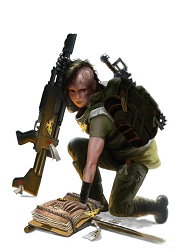
\includegraphics[width=\figwidth]{pics/12/10.png}
	\end{center}
\end{wrapfigure}
Twitch had been driven to a significantly higher-than-usual level of paranoia by the news that he'd be sharing the ship with a Tyranid. 
This was compounded by the ban on indiscriminate booby-traps that Sarge had enacted after several of the acolytes had gotten themselves injured. 
The cherry on top, and primary focus of Twitch's complaints, was the fact that Doc had refused to move back into the barracks after his legs had finished healing. 
Doc claimed his preference for sharing quarters with his hospitalier girlfriend wasn't a slander on the quality of Twitch's defences, but the demolitions trooper didn't buy it. 
He interpreted this decision in the same way he did most things, as a complex conspiracy to make him unhappy.

Finally bringing up the rear of the little parade of misanthropy, was Aimy, who had perhaps the pettiest gripe of all of us: 
her hair was messed up. 
Doc's girlfriend had done a wonderful job of repairing the second set of facial burns our markswoman had received, and she'd used some special hospitaller trick to repair Aimy's scalp. 
Unfortunately, Aimy was completely fixated on the fact that the treatment had left a hand-wide stripe of pure white running through her, now buzz-cut, hair. 
None of us really knew why she cared so much, Aimy hadn't been particularly vain in the past, it was odd that this specific thing loomed so large. 
Perhaps it was because Nubby had the poor taste to say it made her look like a skunk.

The three troopers shared their displeasure with just about everything they ran into, whether it was a minor warp beastie, mutant krootoid, or newbie tech-priest. 
Aimy particularly took grim delight in asking every Acolyte she saw if they thought her hair looked funny, then doing mean things to anyone who gave the wrong answer. 
There wasn't a right one. 
By the time we were nearing our rendezvous their antics, as well as the rest of the team's general attitude, had reached such a level that the Captain actually took notice. 

\begin{wrapfigure}{O}{\figwidth}
	\begin{center}
		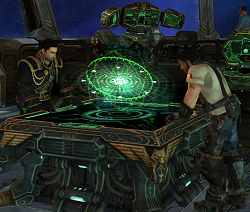
\includegraphics[width=\figwidth]{pics/12/11.png}
	\end{center}
\end{wrapfigure}
It took a bit of work for Sarge to placate the Captain, even though the man was ex-Navy and should have automatically understood the situation. 
Sarge didn't have any trouble getting across that most of our squad had an especially strong dislike for fighting tyranids, and pyskers for that matter. 
The problem was that morale is a far different thing on a ship than it is in a trench, so the Captain didn't see why that excused our behavior.

Sarge eventually managed to explain that while veteran Guardsmen can handle just about anything on the battlefield, they have relatively few coping mechanisms for dealing with slowly impending doom. 
He asked if the Captain would prefer to have us staggering around blind drunk or taking a more "proactive" approach to staying alive. 
The Captain agreed that a bit of complaining and misbehavior was better than Twitch manufacturing reason why we couldn't complete the mission.

In the end Sarge promised that we'd be ready for action when the time came, and quietly hoped like hell that he was telling the truth. 
Luckily, it turned out he was: 
on the final day of our warp travel everything started coming together.

The first break was when Tink and Fio successfully managed to put the largest servitor on the ship into stasis. 
Actually it was originally the second largest servitor, but the overlapping fields had gotten out of sync on the previous test and messily rearranged that hierarchy. 
Anyway, the test was such a resounding success that they hauled the whole thing down to the Cells and crammed Fumbles into it before anyone could stop them.

Aside from how long it took them to safely get our Psyker back out of there, the live test went perfectly. 
Fumble's aura completely vanished when the field was activated and everyone working in the Cells cheered. 
Even Jim seemed happy, despite the way he was chivvying his Acolytes out of the room and explaining that they were definitely not seeing a Tau or a techno-heretical stasis device.
\begin{wrapfigure}{O}{\figwidth}
	\begin{center}
		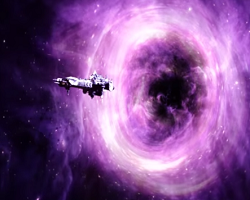
\includegraphics[width=\figwidth]{pics/12/12.png}
	\end{center}
\end{wrapfigure}
The news that we'd be transporting a stasis-ed Tyranid psyker, as opposed to one that was actively trying to kill us, perked everyone up. 
All of us set aside our little distracting grievances as our warp voyage ended; 
well, except for Aimy and Twitch that is. 
The demolitions trooper's behavior wasn't surprising, but the fact that Aimy had to be restrained from beating Nubby to death with the bottle of hair-dye he acquired for her was worrying. 
Fortunately neither of their Obsessions prevented them from prepping for battle, and everyone was ready to kick some ass when we finally reached our destination.

When I say we were ready for action, I mean it: 
we were literally standing in the shuttle bay when the Occurrence Border came out of warp. 
The Space Marines weren't going to catch us sitting around and asking for five more minutes before the mission, no siree. 
So it was sort of awkward when there wasn't anyone at the rendezvous.

We stood in the bay for an hour before we gave up in disgust. 
While the rest of us wandered off, muttering blasphemous remarks about the Emperor's Angels of Death and their idea of punctuality as we did so, Sarge headed up to the bridge to see what the hell was going on.

We'd really expected to find the Marines there ahead of us, it's not like we had a very fast ship. 
We'd even entertained the faint hope that they'd already have the Zoanthrope tied up and ready for us. 
Either way it'd be a matter of in-and-out before the Nids even realized we were there, at least that's what we hoped. 
It was rather unsettling to find ourselves sitting absolutely alone at the far edge of a hostile system. 
It didn't stay unsettling for long though: 
when we took a look around and saw just how hostile the system was, we bumped the situation up to outright terrifying.
\begin{wrapfigure}{O}{\figwidth}
	\begin{center}
		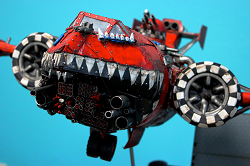
\includegraphics[width=\figwidth]{pics/12/13.png}
	\end{center}
\end{wrapfigure}
Now, we'd all read Oak's orders. 
It was obvious that the system would be a battleground: 
not even Marines are suicidal enough to try this sort of thing in a wholly Tyranid controlled system. 
None of us had been optimistic enough to bet on finding a system that was being cleansed by a massive Imperial fleet, but we'd hoped that our destination would be some Imperial frontier world that just wasn't on our maps. 
Preferably one that had just been reinforced by a few regiments of Guard, and was fighting off a VERY small splinter fleet.

Of course if we couldn't get a world with more Guardsmen than Nids, we'd have happily settled for any Imperial presence, regardless of how many bugs there were. 
Hell, we would have been happy with one of those weird independent systems you get out here, or even a Tau world, so long as they were busy with the Nids. 
All we'd really wanted was a system where the fight was sort of even, and one side wouldn't be shooting at us. 
Instead, what we saw when the Occurrence Border's scanners came online, was four planets, four hiveships, and thousands, if not millions, of far-smaller ships. 
A closer inspection revealed that the little vessels were inorganic and that they were attacking the hiveships with mixed success. 
Sarge left the bridge shortly after the first detailed scans came in.

Sarge came down and gave us the bad news, it was something we needed to know after all, but he took the precaution of stopping at the medbay on the way down. 
Even with the heavy tranq and the Hospitaller's help, Twitch nearly managed to escape into the ship's pipework before Sarge finished telling us about the little ships. 
They hadn't been Imperial or Tau fighters, or even Eldar for that matter. 
Every single one of the smaller craft had been a ramshackle contraption held together by a combination of spit, red paint, and a complete refusal to understand, or even acknowledge, the laws of physics.

Orks? 
Why'd it have to be Orks?
\begin{wrapfigure}{O}{\figwidth}
	\begin{center}
		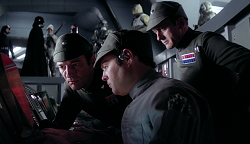
\includegraphics[width=\figwidth]{pics/12/14.png}
	\end{center}
\end{wrapfigure}
The Occurrence Border spent the next few days being as still and quiet as it possibly could. 
Meanwhile, everyone inside it ran around in frenzy of preparation that put our earlier efforts to shame. 
None if it was directed towards improving the Zoanthrope Containment Area any more though, instead it was all focused on keeping us alive long enough to capture the bloody thing. 
Armsmen drilled on repelling boarders, the ship's lances were brought up to as close to functional as they'd ever been, and Tink finished getting everyone equipped with pulse weapons while Fio put the final touches on Spot 2.0. 
The rest of us trained with our new weapons, and kept Twitch from doing anything crazier than usual.

On the third day we were all called up to the bridge by the Captain. 
Well, actually only Sarge and the adepts were called, but the rest of us were tired of all the horrible waiting. 
A very brief message telling us to hold position and wait for secure comm contact was replayed for us. 
The Captain told us he hadn't seen any other vessels enter the system and didn't even have a hard source for the comm message, just a vague direction. 
That was rather disturbing, but no one except Twitch could figure out a way it could be a trap. 
The Captain and Sarge decided to wait and see what happened next.

After half an hour another message came in. 
An incredibly deep voice that practically screamed "Space Marine" identified itself as Sergeant Gravis of the Emperor's Scythes, and instructed us to lower our shields so he could dock. 
As the Captain did so, Sarge squared his shoulders and picked up the Vox's handset, only to have the officer manning it tell him that we still didn't have a target for a secure channel. 
The man asked Sarge if he should just broadcast generally, and Sarge agreed. 
He got about halfway through introducing himself before the Marine voxed back, and told him to cease broadcasting before he alerted the whole system.
\begin{wrapfigure}{O}{\figwidth}
	\begin{center}
		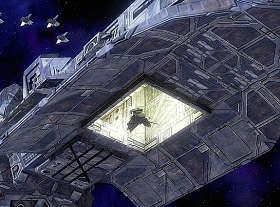
\includegraphics[width=\figwidth]{pics/12/15.png}
	\end{center}
\end{wrapfigure}
Sarge sheepishly hung up the vox, and vented some frustration by asking the communications officer what he meant by "still didn't have a target." It was quickly revealed that sensors still hadn't detected the Marines' ship, despite it being close enough to worry about docking. 


The sensor techs claimed that the incoming ship must be shuttle-sized and have some good stealth systems, but they were sure to spot it when it requested final docking instructions. 
Tink not-very-quietly suggested that, instead of Marines' ship being really stealthy, the techs' systems were just complete shit. 
He then volunteered to have them upgraded to "modern standards" after the mission. 
The ensuing argument was brought to a halt by the Marine voxing again, and telling us to reactivate our shields and close the shuttle-bay doors.

While most of us laughed at the sensor techs for not spotting a ship before it landed on us, Doc raised the question of where the Marines had landed; 
we hadn't actually opened any bays yet. 
Unsurprisingly, given that they were the ones who'd patrolled the ship the most, Nubby and Twitch figured it out first; 
both troopers screamed at Sarge to stop the Marine. 
Sarge and the Captain both caught on to what had happened at the same moment that the techs pinpointed the Marines' ship in the foremost bay on the top of the Occurrence Border. 
The one in the badly warp-tainted area near the prow, which was left open and airless at all times, and was NEVER to be used.

The two normally stoic men frantically ran towards the communication officer and screamed at him to open a channel. 
In the background a confused sounding comm came in from the Marine, asking why everything was so green and why there was a crewman without a void-suit in the airless bay.

Sarge won the sprint, and had the vox halfway to his mouth when the Marine's confused questions changed to reports of incoming hostiles.
\begin{wrapfigure}{O}{\figwidth}
	\begin{center}
		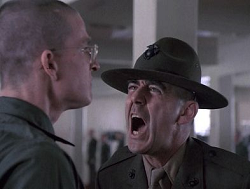
\includegraphics[width=\figwidth]{pics/12/16.png}
	\end{center}
\end{wrapfigure}
Despite everything that happened afterwards, Sarge's reaction was about as perfect as was possible. 
In his best noncomm voice, he bellowed at the Marine to disengage and pull his shuttle out of the bay. 


I'm not sure if you're familiar with how big and loud a Space Marine's voice is, but overriding one via pure volume and vitriol is a feat worthy of legend. 
Every time the Marine tried to argue, or ask for clarification, Sarge just shouted over him in that parade-ground voice he'd spent his life perfecting. 


It was working and everything might have turned out fine, if there hadn't been a second Marine that is. 
The other Astartes, who'd been spared the full brunt of Sarge's wrath, cut in and asked his battle-brother if he'd tarnish the Chapter's honor by running like a squad of guardsmen without a commissar. 
The first Marine rallied, and announced his intention to enter the bay and deal with the hostiles that were evading his shuttle's weapons.

Sarge switched tactics and frantically tried to explain that there weren't any enemies and opening the airlock would let the warp-fungus in, but dissolved into furious cursing when he heard the shuttle's lock cycle. 
With a final growl of "This isn't a battle you idiot, it's sanitation. 
You're going to get yourself killed fighting fungus" he handed the vox unit over to Doc and the adepts.

Doc and everyone else with more charisma than a dead felid slowly explained the situation to the marine that hadn't just contaminated himself. 
The rest of us just stood there and listened to the sound of a Space Marine trying to kill xenos that miraculously seemed to dodge every shot. 
Nubby and Aimy started placing bets on how long it would be before the warp-fungus, as we called it, ate through the Marine's power-armor, and whether the Marine would even be able to notice. 
No one gave him good odds: 
we all knew just how nasty the warp-fungus could get. 
Hell, it'd been some of us who first discovered the stuff.
\begin{wrapfigure}{O}{\figwidth}
	\begin{center}
		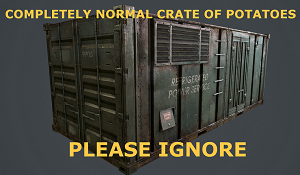
\includegraphics[width=\figwidth]{pics/12/17.png}
	\end{center}
\end{wrapfigure}
Standard operating procedure on the Occurrence Border was to just seal off any warp-tainted sections with nothing important inside. 
The lack of anything living to mess with kept the number of manifestations to a minimum, and anything that did appear usually faded before it could claw through the sealed bulkheads. 
Occasionally though, something nastier than usual would appear and need dealing with. 
Nubby, Twitch, Fumbles, and recently Aimy, spent a lot of time watching for signs of this sort of stuff, and often got stuck with the job of fixing it.

Anyway, the warp-fungus was one of those nastier than usual things, but fixing it had been a bit of a problem. 
Fumbles had sort of "heard" it in the tainted shuttle bay months ago, back before we'd reached the Tau border worlds in fact. 
He'd made such a fuss about the psychic noise it was emitting, that Nubby and Twitch had agreed to risk a recon mission into the bay between warp-jumps. 
They'd run in, and pinpointed a large container labelled "Potato Substitute: 
15 Tonnes" as the source of the noise. 
Because they were relatively savvy to how this sort of things worked, they'd declined to actually open the container, and just solved the problem in the same way they'd solved most of the others. 
Which is to say they covered it with detpacks.

At the time they'd declared victory when the explosion went off and the psychic noise stopped, but in retrospect that had only served to spread the fungus all over the bay. 
While the noise hadn't returned, patrolling armsmen began reporting strange sounds then disappearing, and then other armsmen reported hearing or seeing the missing ones. 
Over a dozen had vanished into the bay before Nubby and the rest took a second look. 
They'd found it covered with the fungus, which was in the process of dissolving everything less sturdy than the bay's blast-proof outer doors and walls. 
Also, it was filled with the missing armsmen, who were beckoning them inwards.
\begin{wrapfigure}{O}{\figwidth}
	\begin{center}
		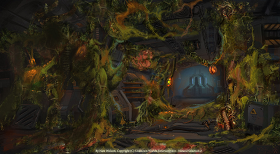
\includegraphics[width=\figwidth]{pics/12/18.png}
	\end{center}
\end{wrapfigure}
Nubby, Fumbles, and Twitch had immediately shut the door and ran for it. 
As the they'd fled, a horde of Orks, Gensestealers, and a few other varieties of xenos appeared at the end of the hall and blocked their escape. 
Fortunately Fumbles was along and realized that the new enemies were some sort of psychic illusion. 
The psyker was able to dispel the illusion without anything more serious than a temporary reversal of gravity happening, and the debatably-heroic trio escaped.

There'd been a few attempts to kill off the warp-fungus after that. 
Unfortunately between its caustic nature, the hallucinations, and the fact that it was hellishly hard to kill, all that was accomplished was getting a few more armsmen and a whole lot of servitors melted. 
Eventually someone suggested just voiding the bay, then leaving it open until the stuff died. 
That didn't actually work, but it did cause the stuff to go dormant unless something ventured into the bay. 
Since we didn't actually use the bay for anything, the Captain had decided that the problem was no longer pressing and we'd gotten back on our way. 


As a precaution Ol' Bill had reinforced the seal on all the bay's doors and vents, and the only one allowed to go near it had been one of the senior tech-priests. 
The cogboy had some ideas about chemical sprayers deployed by servoskulls, and Jim said he'd made some real progress, but then the whole tech-heresy thing had come up...

ANYWAY, that's what the Space Marines had just landed in. 
A bay full of psychically active, highly caustic, and incredibly hard to remove warp-fungus. 
Honestly though, it was still only the third worst thing on the Occurrence Border they could have landed in… our ship was definitely a little overdue for a tuneup.
\begin{wrapfigure}{O}{\figwidth}
	\begin{center}
		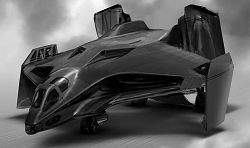
\includegraphics[width=\figwidth]{pics/12/19.png}
	\end{center}
\end{wrapfigure}
Through an absolutely heroic amount of persuasion, Doc and the adepts managed to convince the Marines to abandon the bay. 
The second Marine, who identified himself as Sergeant Rebus, turned out to be very susceptible to logical arguments, and even helped talk Sergeant Gravis around before the fungus was able to melt through his boots. 
We still didn't forgive him for screwing up Sarge's initial attempt though, because even if Gravis was going to be fine, he'd cycled his shuttle's airlock twice in the warp-fungus bay. 
There was no way that bird wasn't contaminated as hell.

We watched as not one, but two shuttles rose out of the bay. 
Neither of them looked anything like the Thunderhawks we'd expected when they told us we'd be working with Space Marines. 
Aside from being incredibly sleek, both of them were completely black, and only visible because of our ship acting as a backdrop. 
One of them was definitely having a little trouble flying in a straight line though, and showed up as a faint ghost on the sensor techs' scopes. 
The other remained stubbornly invisible to all scanners as it settled in space in front of the bridge.

The decontamination process was not fast: 
the sprayer skulls had to be found and refilled, the contaminated shuttle had to be completely voided, and a holding area had to be set up. 
On top of that, the whole time this was going on, Sergeant Gravis and his shuttle's crew were, as Tink put it, tripping balls. 
Given how heavily armed they were, the situation was very uncomfortable, but luckily no one was killed and only one sprayer skull was destroyed.

After hours of tedious cleaning, not to mention angry shouting about who's fault this all was, our team met with the Space Marines in the Occurrence Border's fanciest conference room. 
Our planning session was short, direct, and absolutely terrifying.
\begin{wrapfigure}{O}{\figwidth}
	\begin{center}
		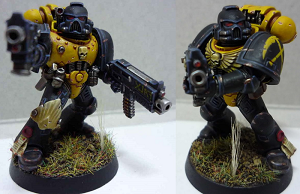
\includegraphics[width=\figwidth]{pics/12/20.png}
	\end{center}
\end{wrapfigure}
Sergeants Gravis and Rebus of the Emperor's Scythes Space Marines Chapter were not what you'd call socialites. 
In fact they were even more aloof than the few Marines we'd met previously. 
They stomped into the conference room still wearing their power armor, and didn't even bother to remove their helmets. 
It was unnerving as hell talking to them, and even Sarge couldn't hold onto his "Inquisitorial Dignity" in the face of those stares. 


Rebus did most of the talking, and started by explaining that there were two main objectives and would be two separate teams. 
The first team would consist of him and his four scouts. 
The second would consist of Sergeant Gravis and his two scouts, one of which would be piloting the shuttle, plus Interrogator Sargent and his five Inquisitorial Guardsmen.

Sarge hesitantly asked if we'd need any support staff in the field. 
This triggered looks of terror from Jim, Hannah, and all of the adepts, but Rebus said that they wouldn't be necessary. 
From the far end of the table, Fumbles held up his hand and asked if he was coming. 
The Marine considered this, then asked if he was capable of using his powers while simultaneously fending off the Hive Mind's continuous psychic assault. 
Fumbles quietly put his hand back down.

After waiting a few seconds to see if anyone else would interrupt, Rebus started explaining what the two teams would be doing. 
Our team would go to the third planet in the system, then find and capture a Zoanthrope; 
his team would destroy the hive ship orbiting it. 
Everyone in the room just sat there and stared at the marines as Rebus started explaining the transportation situation and timeline. 
Tink managed to overcome his shock before anyone else, and loudly asked the marines if they were insane-slash-retarded.

\begin{wrapfigure}{O}{\figwidth}
	\begin{center}
		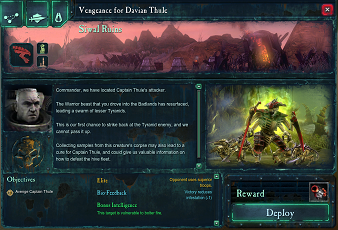
\includegraphics[width=\figwidth]{pics/12/21.png}
	\end{center}
\end{wrapfigure}
Aimy and Nubby snickered, and Doc hastily clapped a hand over Tink's mouth. 
Sarge took a deep breath, and asked Sergeant Rebus to explain why, and more importantly HOW, the marines were going to destroy an entire tyranid Hive Ship.

Rebus met Sarge's stare, and said his Chapter's primary interest in the system was ensuring that the Tyranids did not overwhelm the Orks and form a new splinter fleet. 
Capturing a live zoanthrope for the Inquisition was merely a side-mission, a small favor to be completed when convenient. 
As for how, his team would board the Hive Ship and destroy it from within; 
further details were not for those outside the chapter. 
All we needed to know what that the Ship would die after we captured the Zoanthrope, but before their psi-suppressants could wear off and allow the Hive Mind to destroy the beast.

As everyone digested this, Twitch broke his remarkably long silence. 
The demolitions trooper volunteered that the Marines probably had a vortex bomb, since an explosive would merely scatter still-living pieces of ship across the planet, and a poison or virus would require a lot of sampling plus a nearby laboratory. 
Both Marines glared at Twitch, who ignored them and went back to fiddling with the mine he was holding.

After some more awkward silence, Sergeant Rebus went back to explaining the mission details. 
Both teams would deploy in his stealth shuttle, since the warp-fungus had gotten into the control systems of Gravis'. 
First we'd insert his team on the hive ship, and then go down to the planet and capture the Zoanthrope. 
The Occurrence Border would follow us in on low power and stop at the edge of the Hive Ship's Shadow, where it could easily warp out in an emergency. 
If our mission went quickly we'd return to it and drop off our prize before the shuttle extracted  Rebus' team, otherwise we'd pick them up on the way back.
\begin{wrapfigure}{O}{\figwidth}
	\begin{center}
		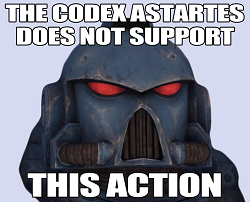
\includegraphics[width=\figwidth]{pics/12/22.png}
	\end{center}
\end{wrapfigure}
It slowly dawned on us that the Marines' plan called for us to sit, as helpless passengers, in a shuttle that would not only be carrying a notoriously unstable warp-weapon, but would also be closing to boarding range with a Hive Ship. 
Even without the swarm of Ork Fightas attacking the ship, and the fact that we might be making a second visit while that warp-weapon was actually armed, it sounded incredibly dangerous. 
With them, not to mention the whole capturing a xenos psyker thing, it sounded downright suicidal.

While the rest of us silently panicked, Doc hesitantly asked if it wouldn't make more sense to use both of the Marines' shuttles. 
Gravis, whose armor was sporting some truly impressive acid burns, glared at Doc and swore loud enough that we could hear him despite the fact that he didn't have his helmet's speakers on. 
He bitterly suggested that we should have thought of that before neglecting the maintenance of our ship's shuttle bays, and then fell back into his sullen silence. 


Doc soldiered on despite this rebuttal, and asked whether the mission could be delayed until our tech-priests fixed the fungused shuttle. 
Jim and Hannah made some panicked gestures, which seemed to imply that they had no idea how the stealth-shuttle even worked, much less how to fix it. 
Rebus ignored them, gave Doc a simple "No", and announced that the briefing was over. 
We'd be leaving as soon as his Scouts finished transferring equipment to the shuttle and Gravis' field repairs were completed. 
One of Gravis' scouts would deliver our mission-critical gear and explain the capture procedure to us in the meantime.

With that the two Marines stomped out. 
One by one the Enginseers, adepts, and Fumbles followed them, leaving only us guardsmen sitting there, feeling like we'd lost all control of the situation.
\begin{wrapfigure}{O}{\figwidth}
	\begin{center}
		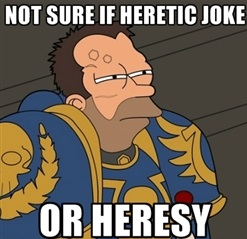
\includegraphics[width=\figwidth]{pics/12/23.png}
	\end{center}
\end{wrapfigure}
Now, we'd felt out of our depth before. 
Hell that'd been our default state of mind since the Inquisition drafted us. 
This was worse than usual though: 
the Marines had left us feeling like children. 
It wasn't embarrassment over the shuttle thing, that was at least as much their fault as ours, it was just that we felt incredibly outclassed by the three meter tall killing machines.

It was odd that the two Marines were so daunting, since as Twitch pointed out, we'd actually killed three Chaos Marines during our missions. 
Doc suggested that the issue was that they were on our side. 
The ones we'd killed were vile traitors deserving of nothing but scorn and death, but these two were physical manifestations of the Emperor's divine wrath. 
Or to put it more simply, we couldn't compensate for our discomfort by trying to kill them.

Twitch was half-way through suggesting that shooting the Marines just a little would make us feel better, when Gravis' Scout came in. 
That was a very awkward moment, but the Scout eventually accepted that it was just a little joke. 
None of us would even consider doing such a thing, and we certainly didn't dedicate large amounts of our time to planning complex betrayals of our allies. 
Well unless they were Eldar. 
Or tech-priests. 
Or deserters, cultists, hereteks, annoying Interrogators, commissars, rogue traders, rival Inquisitorial teams, or people who might be Orks in disguise. 


But since Marines and their Scouts were none of these things, there was obviously nothing to worry about. 
Unless they really WERE Orks. 
They were much bigger and musclier than normal people after all...

Sarge put a stop to Twitch's newest paranoid fantasy before it got started, and asked the Scout what was in the crates on the pallet he was pushing. 
The Scout eyed us all dubiously, and said it was our Grav-Chutes.

All of us digested the horrible implications of those two words and went quiet. 
Except for Nubby that is, who was a little slower on the uptake.
\begin{wrapfigure}{O}{\figwidth}
	\begin{center}
		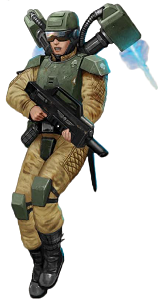
\includegraphics[width=\figwidth]{pics/12/24.png}
	\end{center}
\end{wrapfigure}
\greentext{>Grav-whats?}


Chutes

\greentext{>What-shoots?}


Grav-Chutes!

\greentext{>What-whats?}


You're guardsmen, you must know what Grav-Chutes are! 
You know: 
small, backpack-size anti-gravitic devices that allow Imperial troops to float safely to the ground on a column of anti-gravitic force from any height in a world's gravity well, including sub-orbital heights.

\greentext{>Ohhhh you mean screamy-fally-deaf-packs. Yea we're familiar wif dose. Whatchu doin with em? Cause I know a guy who knows a guy...}


They're for you to deploy from the shuttle with. 
You just said you're familiar with them, surely I don't need to draw you a picture.

\greentext{>What? Are you mental? When I say "familiar" I mean we've pulled a buncha dem off deaders. None of us 'ave ever used one; you can tell, 'cause we're not pancake-shaped.}


That's unfortunate, you have two hours to learn how to operate one. 
I'll assist in your training, is there a nearby cargo bay or lift shaft we can use?

\greentext{>Sahhhhge, the baby Space Marine is tryin ta kill us Sahge. Why's everyone always trying ta kills us Sahge? }


\begin{wrapfigure}{O}{\figwidth}
	\begin{center}
		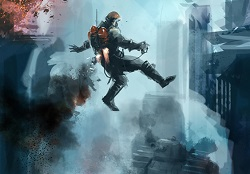
\includegraphics[width=\figwidth]{pics/12/25.png}
	\end{center}
\end{wrapfigure}
The best term for our training with the Grav-Chutes was Crash Course. 
The Scout Marine made sure our chutes were on, walked us to the edge of the shaft, then pushed us off. 
He claimed it was how he'd been trained, and the man evidently saw no reason why non-superhumans should learn any differently. 
Sarge didn't let anyone argue, there wasn't time.

None of us enjoyed the experience of being thrown into a lift shaft with nothing but an underpowered anti-grav unit and a pair of tiny thrusters between us and pancakey-death. 
It's hard to say who did the worst: 
it was pretty much a three-way tie. 
Doc had so little control that he got stuck on a light fixture, and had to be rescued by the Scout Marine. 
The humiliation of being suspended by his pants half-way up the shaft was slightly overshadowed by the way that the Scout had just cut them off, and then insisted he keep practicing instead of getting a new pair. 


While the Scout was busy with Doc's rescue, Tink decided that he could convert his chute to a full jump-pack using some of the techniques he'd picked up working on his drone. 
It turned out he was wrong; 
so much so in fact, that he had to be issued the only spare chute. 
Of course, Tink immediately declared that he knew what he'd done wrong, and started to retry the modifications using his replacement chute. 
Sarge had to take his tools away.

Finally, Aimy misinterpreted a suggestion to wear a helmet as a comment on her hair. 
She tried to deck the Scout, and found out a Space Marine's jaw is a lot tougher than any non-augmetic hand. 
Doc, still pantsless, checked her hand and said it wasn't broken, so Aimy grumpily resumed her training. 
For his part, the Scout Marine took the irrational attack in stride, but that was obviously the point where we lost the last of our credibility in his eyes.
\begin{wrapfigure}{O}{\figwidth}
	\begin{center}
		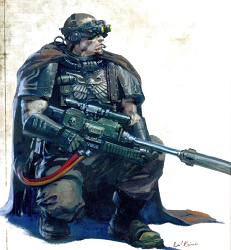
\includegraphics[width=\figwidth]{pics/12/26.png}
	\end{center}
\end{wrapfigure}
Despite all the difficulties and our teacher's disgust with us, we all managed to get down the shaft safely a few times before the training ended. 
We gathered up our gear, got Doc some new pants, and made our way to the bay where the un-fungused stealth shuttle was being prepped. 
Once there the Scout Marine brought out an impressively large sniper rifle and explained how the Zoanthrope's capture would work. 
We noticed that unlike the previous lesson, this briefing consisted of nothing but short words and included a lot of hand gestures as well as a few pictures. 
None of us commented, but Aimy and Tink were obviously taking note of every little implied insult.

The gist of the plan was that the stealth shuttle would sweep over the battlefield until we saw a Zoanthrope. 
The shuttle would fly over the target, and then everyone but the pilot would deploy via Grav-Chute. 
From there, speed was the name of the game: 
the estimated mission length was ten minutes if our insertion was undetected, and three if it was. 
If we took any longer, Tyranid reinforcements would bury us.

Our squad would secure a perimeter, and hold it against any tyranids that came to support the Zoanthrope, while Sergeant Gravis wore down the xenos' pyschic-shield-bubble-thing. 
Once the shield was breached, the Scout would shoot the Zoanthrope with a specially tailored sedative and psi-suppressant, and then we'd all fall back to the nearest possible landing area for extraction. 


It was the complete opposite of all the horribly complex ops we'd suffered through since joining the Inquisition: 
it was ultimate simple, straightforward plan. 
If it wasn't for the fact that we'd be outnumbered thousands to one, we'd have loved it. 
As it was though, there's no word for how much we hated that plan.

Honestly all of us, even Sarge, would have bailed if the two Space Marines hadn't shown up. 
None of us had the nerve to refuse the Astartes, so we boarded the shuttle and headed off to our certain deaths.
\begin{wrapfigure}{O}{\figwidth}
	\begin{center}
		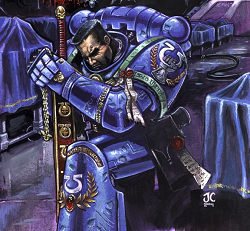
\includegraphics[width=\figwidth]{pics/12/27.png}
	\end{center}
\end{wrapfigure}
The shuttle trip into the system was amazingly unpleasant. 
It wasn't that the stealth shuttle was crowded: 
there were only thirteen of us in it, or fifteen if you counted the seats taken by Spot and the Vortex Bomb, and the seats themselves weren't that bad either. 
Sure they were a little on the big side, but Space Marines definitely spare a bit more budget for comfort when building a ship than the Guard does. 
So the ship was fine, the problem was the atmosphere being generated by our fellow passengers. 
They were too quiet. 


See, if it were a Guard shuttle everyone would've been complaining, joking, or smoking. 
Even the dryest Inquisition teams we'd been assigned to would've at least been doing some gear checks, or reminding us stupid guardsmen what our job was. 
The marines and their scouts just sat there and silently prayed or meditated or something. 
No talking, no moving, and hardly any breathing for hours upon bloody hours. 
You'd think we could just ignore it, but any time one of us made the slightest bit of noise the entire creepy lot would glare at us like, well, like noisy children in a chapel.

The silence wore on our nerves. 
There was nothing to do but think about the upcoming mission or stare at the ominous bulk of the Vortex Bomb, which was making the sort of unhearable noises we associated with a weak gellar field. 
We were all reaching our limit, and it was race to see if Twitch or Aimy would snap first, when Sarge decided that politeness was overrated. 
He commandeered one of Twitch's camo-tarps and hung it across the shuttle interior, walling away all the creepy super-humans except for Gravis' Scout. 
The big guy tried to glare us down by himself as we all started being as noisy as we damn well pleased, but we had him outnumbered, and Sarge threatened to put a second tarp over him if he kept it up.

\begin{wrapfigure}{O}{\figwidth}
	\begin{center}
		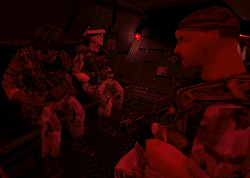
\includegraphics[width=\figwidth]{pics/12/28.png}
	\end{center}
\end{wrapfigure}
The remainder of our approach to the Tyranid hive ship was spent the usual ways. 
Tink tinkered with Spot 2.0, removing the overweight-skull-probe disguise and trying to get a few of the systems he and Fio hadn't finished kludging together functional. 
Doc wrote his usual soppy "if I die on this mission" letter to his girlfriend, while Aimy and Nubby read over his shoulder and made unhelpful suggestions. 
Twitch muttered to himself as he imagined hundreds of scenarios involving Tyranids and Orks. 
As his mind ran in it's crookeder-than-usual circles, he continuously moved gear and explosives between his bag and the massive pile of spares he'd brought. 
Sarge watched as we frittered away our time, and saw that it was good. 


We all suffered a moment of heart failure as Sergeant Rebus tore down the tarp, followed by another when the homemade cluster-mine Twitch had been holding hit the floor. 
The Space Marine stood there and waited while we picked springs and, thank-the-Emperor unarmed, explosives out from under our seats. 
When the last bomblet had been collected, Rebus informed us that the shuttle was nearing the hive ship and would be switching to full stealth mode. 
We were to secure ourselves and our gear, put on our rebreathers, and stay out of his team's way while they deployed.

We did as ordered, and a few minutes later the shuttle ride went from boring to terrifying. 
The cabin switched to emergency lights, the air vents stopped blowing, and the gravity deactivated. 
We floated in our seats for a few seconds, then the first "evasive maneuver" hit us. 
Let me tell you, no one thinks about those grav tied to a shuttle's engines seriously until they're turned off. 
Instead of the usual little jolts of spillover, they were as long, continuous pulls in seemingly random directions. 
We felt completely helpless as we bounced and swung in our crash harnesses, then Tink decided it might be better if we could see what was coming and anticipate the maneuvers. 
It was not.

\begin{wrapfigure}{O}{\figwidth}
	\begin{center}
		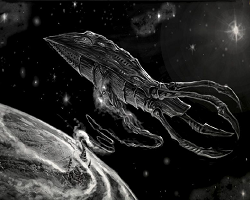
\includegraphics[width=\figwidth]{pics/12/29.png}
	\end{center}
\end{wrapfigure}
Who knows what the Marines and Scouts thought when Spot 2.0 drifted past them and entered the cockpit, they didn't actually say anything about it, and were already glaring at us for how loudly we were complaining about the turbulence. 
Anyway, they seemed just as interested as us when Tink projected the drone's vid feed on the front bulkhead.

We all stared at the image of the massive Tyranid bioship looming in front of us, and then at the smaller shapes swarming around it. 
It was hard to say if there were more Ork Fightas or Tyranid fliers, and either way there was a constant stream of reinforcements rising from the planet and spewing from the Hive Ship. 
It was complete chaos: 
the space around the hive-ship was filled with rokkits, shells, bio-plasma, pyro-acid, and millions of tonnes of wildly spinning debris; 
and for some reason, we were flying right into it.

Bloody Space Marines.

All of us just sat there and stared, and then we saw the cause of one of those evasive maneuvers. 
A speck suddenly grew into a Fighta, and then zipped past by such a thin margin that we could see the Ork piloting it. 
A split second later it was followed by a stream of bio-plasma and a Tyranid interceptor. 
Doc swallowed, Twitch whimpered, and Aimy swore.

Variations of that scene repeated dozens of times as we closed with the Hive Ship. 
It's hard to say which was more amazing: 
the way the Scout Marine pilot twisted away from every impact with bare meters to spare, or the fact that none of the hostiles saw our shuttle, even while nearly colliding with it. 
Our slow approach to the Hive Ship through that space battle was a terrifying and humbling reminder that, if Guardsmen's nerves are steel, Space Marines' are Adamantium.

Not that we actually had what you might call Nerves of Steel, all of us were scared shitless. 
And when the pilot took cover from a pyro-acid barrage behind a Landa that was visibly filled with Kommandos, Twitch went from scared to full on Freaking Out, Man.

\begin{wrapfigure}{O}{\figwidth}
	\begin{center}
		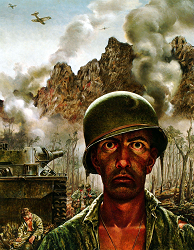
\includegraphics[width=\figwidth]{pics/12/30.png}
	\end{center}
\end{wrapfigure}
When Twitch started gibbering Sarge barked orders at Tink and Doc to turn off the projection and prep a tranq, but none of us had anywhere near the same speed as the panicked demolitions trooper. 
In a startlingly short amount of time, Twitch had cut his way out of his crash harness, and relocated to a "more defensible position," leaving a trail of detpacks floating the air behind him. 
Said defensible position turned out to be the small amount of space between the Vortex Bomb and the seat that held it.

Sarge immediately undid his own restraints and launched himself across the shuttle, only to wind up pinned against a pair of unhappy Scout Marines as the pilot evaded something or other. 
A rain of detpacks landed on everyone on that side of the shuttle, Guardsman and Marine alike, and Sergeant Gravis decided that enough was a enough. 
The Space Marine's boots adhered to the floor with a deep clang as he left his seat. 


Most of us watched in amazement as the Space Marine slowly stomped across what the shuttle's acceleration meant was actually a wall. 
Twitch though, was too busy with his paranoid panic attack to notice, until a massive hand snapped out pulled the detonator from his grip, that is. 


Sergeant Gravis had probably thought that removing the detonator would neatly, er, defuse the situation. 
He was completely wrong of course, but the theft did focus Twitch's attention on him instead of imaginary Kommandos. 
Unfortunately, that attention took the form of a thrown object, which adhered to the Space Marine's hand when he tried to bat it away.

\begin{wrapfigure}{O}{\figwidth}
	\begin{center}
		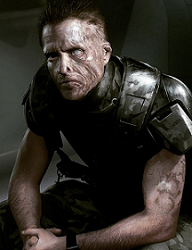
\includegraphics[width=\figwidth]{pics/12/31.png}
	\end{center}
\end{wrapfigure}
We could practically hear the gears in Sergeant Gravis' head whirring as he registered the detpack stuck to his palm and the two detonators which had practically materialized in Twitch's hands. 
The giant in the acid-pocked armor stared into the wild eyes of the demolitions trooper who was currently lying across a Vortex Bomb and accusing him of being One Of Them, and decided that intimidation and force were not viable options. 
So, in the gentlest voice a half-tonne hybrid of man and tank can manage, he tried reason.

Gravis started by asking Twitch to calm down, that worked about as well as you'd expect. 
The Space Marine then tried explaining that there were no enemies in the shuttle, everyone here was Twitch's ally. 
Twitch's responded by chucking another detpack at him and screaming "THAT'S WHAT THEY ALL SAY, THEN THE MASK COMES OFF!" This seemed to confuse Gravis, so Doc helpfully explained that he'd just been accused of being an Ork in disguise. 
Gravis pointed out that Twitch was obviously insane, which won him yet another detpack and a scream of "THEY ALL SAY THAT TOO!"

At that point Gravis must have been losing confidence in his strategy, because he turned as asked the rest of us what to do. 
Nubby, Aimy, and Tink all simultaneously made unhelpful suggestions, and Sarge was busy clinging onto Sergeant Rebus' seat as yet another evasive maneuver tried to fling him across the shuttle. 
Doc told the Marine he was doing fine: 
this sort of argument was pretty much the standard operating procedure if no one managed to tranq Twitch before he got the explosives out. 
He suggested that Gravis continue by taking off his helmet and proving he wasn't an Ork. 
Twitch agreed that the Ork should show us his real face. 
So he did.

Tink's shout of "WHAT HAPPENED TO YOUR-" was cut off by Doc's hand. 
Aimy cackled, until Nubby pointed out that the Marine still had most of his hair. 
Sarge asked what was going on, and Twitch admitted that Gravis wasn't an Ork. 
Probably.

\begin{wrapfigure}{O}{\figwidth}
	\begin{center}
		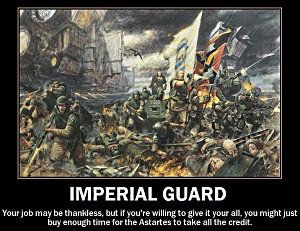
\includegraphics[width=\figwidth]{pics/12/32.png}
	\end{center}
\end{wrapfigure}
In the incredibly awkward silence that followed, Sergeant Gravis put his helmet back on, his Scout Marine glared at us, and Twitch asked if someone would help him off the Vortex Bomb. 
He was stuck.

Gravis collected both Twitch and Sarge, who was still clinging to the meditating Sergeant Rebus for dear life, and deposited them both in their seats. 
As the Marine stomped around, he talked to us, giving us a morale boosting lecture he claimed was given to him as an acolyte on his first boarding mission. 
We were instructed not to worry about what we couldn't control, and to focus on remember glorious victories of the Chapter, or in our case, the Cadian Regiments. 
Nubby asked what was so special about those nutters. 


This caused a pause in the motivational speech. 
It was eventually established that our regiment wasn't from Cadia, Catachan, Krieg, Elysia, Maccabeus, Mordian, Tallarn, Vostroya, or any other world famous for it's contribution to the Guard. 
Furthermore our regiment had never accomplished anything other than serving as cannon fodder for more important Imperial Forces. 
No glorious victories for us.

At an indignant objection from our markswoman, this was adjusted to: 
"No glorious victories for anyone except Aimy and her Nobby Regiment of Nobby Nobs."

Sergeant Gravis stared at us, then asked what in the Emperor's name we were doing in the Inquisition. 
Sarge sighed, picked at a stray detpack which had adhered to his sleeve, and admitted that not a day went by that he didn't ask himself that same question.

\begin{wrapfigure}{O}{\figwidth}
	\begin{center}
		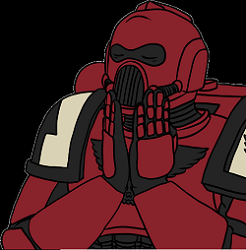
\includegraphics[width=\figwidth]{pics/12/33.png}
	\end{center}
\end{wrapfigure}
The rest of the approach to the Hive ship passed without incident. 
At least as far as us passengers were concerned that is, the pilot definitely had to dodge a whole lot of something over the last few minutes though. 
Thank the Emperor Tink never turned the vid feed back on.

At a word from the pilot Sergeant Rebus and his four Scout Marines sprang out of their seats and positioned themselves around the Vortex Bomb. 
A few moments later there was a squishy impact, and the stealth shuttle's rear door opened to reveal a pulsating wall of flesh-stuff. 
The Scouts painted it with something, Rebus stabbed it with his power sword, and a gap was pried open.

To our disgust, the five-Marine boarding party then smeared themselves with the juices running from the gap. 
Once they, and the Vortex Bomb, were good and covered, they pulled on some Cameleoline Cloaks that looked far better than any that had ever been issued to us lowly Guardsmen, and climbed through. 
Sergeant Gravis planted a probe-looking device in the gap behind them, and then sealed it with some big staple-things and some chemical spray. 


When the gap was closed, we heard Gravis and Rebus do a comm check and schedule the pickup. 
Then the shuttle's door silently closed and we started drifting away. 
From docking to undocking, the whole boarding operation took just under five minutes. 
It the most impressive display of efficient professionalism we'd ever seen, but I'm not sure any of drew a breath during the whole thing. 
We all prayed to Emperor that we wouldn't have to be on the shuttle during their pickup.

There's a moral about getting what you wish for in there somewhere.

\begin{wrapfigure}{O}{\figwidth}
	\begin{center}
		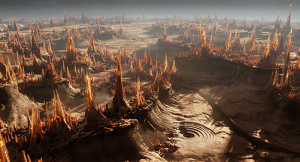
\includegraphics[width=\figwidth]{pics/12/34.png}
	\end{center}
\end{wrapfigure}
We descended to the planet alongside the hail of spores spewing from the Hive Ship. 
It went a lot faster, and required fewer evasive maneuvers, than our approach had, which was good for our frayed nerves. 
Now that Sergeant Rebus and his team of suicidal supermen had departed, Gravis and his scouts became a little more chatty.

The Scout piloting the shuttle brought the gravity up enough to keep us in our seats, and told Gravis that he was starting scans. 
Gravis brought out an oversized dataslate, and began staring at it with the other Scout. 
They didn't seem to think that we really needed to take part in the discussion, but when Tink sent his drone to hover over their shoulders, Gravis decided it was easier just to let us participate.

Gravis and his two scouts were searching the battlefield below us for signs of Zoanthropes; 
specifically they were looking for big-ol bolts of warp-lighting which could be traced back to the xenos psyker firing them. 
That sounds fairly simple, but given how far up we still were and how much of a mess the battlefield was, we decided that it was pointless to try and help. 
While the marines strained their eyes, the rest of us concentrated the sort of things us lowly guardsmen find important, namely weather, terrain, and hostile positions. 
These turned out to be: 
acid rain, wasteland with giant spiky rocks, and everywhere. 
In short, it wasn't a place we wanted to get anywhere near, much less drop onto via grav-chute.

Nubby and Tink started the argument by complaining about the suicidal nature of the mission and suggesting that we just lie on the report, which prompted the Scout Marine to tell us all to grow a backbone and a proper sense of duty. 
Aimy told him where he could stick his backbone and sense of duty, and things went downhill from there. 
Sadly there wasn't time to get a real good fight going: 
we only managed a bit of name-calling and a few anatomically-improbable threats before Gravis finally spotted some warp-lighting.

\begin{wrapfigure}{O}{\figwidth}
	\begin{center}
		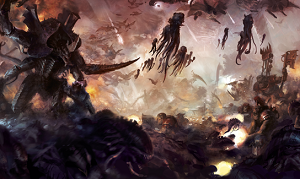
\includegraphics[width=\figwidth]{pics/12/35.png}
	\end{center}
\end{wrapfigure}
Sarge, Doc, and Twitch stared at the dataslate with the Marine. 
The section of battlefield he was looking at was a complete free-for-all between the Orks and Nids, and a particularly dense cluster of jagged rocks was emitting bursts of lighting. 
Gravis said that the frequency of the bolts indicated it was a lone psyker, and went on to point out that the position was not strongly defended against an airborne insertion. 
He suggested that we move on the target immediately, before it was killed or the battle shifted, but Doc and Sarge didn't like that they couldn't see inside the pile of rock the psyker was hiding in, and Twitch was Twitch.

Sarge asked Gravis how sure he was that A: 
there wasn't a whole hive's worth of nids in there and, at Twitch's insistence, B: 
that the lighting-shooting xenos wasn't actually an Ork. 
Gravis just glared at us and said he was 73% certain that this was an acceptable target. 
Our fearless leader tried to stare down the Space Marine for about five seconds, then decided that this sort of decision, not to mention arguing with Astartes, was above his paygrade.

Sarge rounded on the rest of us, and started bellowing orders to prep for deployment. 
Tink got Spot stealthed up and verified that our scopes were synced, Nubby and Aimy flung a final few insults at the Scout Marine, Doc tried to remember which button was which on his Grav-Chute, and Twitch angrily grabbed a last armful of explosives while muttering about no one taking Orks seriously. 
When everyone was ready, we formed up behind Sergeant Gravis and his Scout. 
A few minutes later, the shuttle hatch slammed open.

The Space Marine stepped out into the air and dropped out of sight. 
Sarge followed him to the edge, looked down, and froze as he saw just how far down and covered-with-pointy-things-and-xenos the ground was. 
Then the Scout Marine pushed him.

\begin{wrapfigure}{O}{\figwidth}
	\begin{center}
		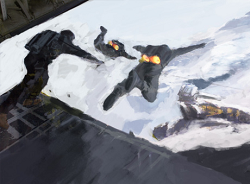
\includegraphics[width=\figwidth]{pics/12/36.png}
	\end{center}
\end{wrapfigure}
Now, just to be clear, while there are entire regiments of Guardsmen dedicated to doing grav-drops, the rest of us think they're insane. 
Even your average Catachan will call an Elysian, or any other type of drop-trooper, an adrenaline-hungry madman. 
And mind you, that's coming from someone who would gleefully try to kill a Warboss with nothing but a combat knife. 
I mean, who in their right mind flies all the way to the battlefield in a perfectly functional shuttle, then jumps out of it while it's still half a klick off the ground? 


Anyway, dropping through the air towards a pile of rocks that resembled nothing so much as a giant daemonic hedgehog was not on the list of things we'd joined the Guard to do. 
The fact that there was a hostile psyker inside said rocks, not to mention the bloody melee of Orks and Tyranids around them, did not make it any more attractive. 
If it wasn't for the fact that Sergeant Gravis was already on the ground and clearing our landing area, we all would have stayed in that shuttle. 
Also the Scout Marine kept pushing us.

Despite how unpleasant we found the drop, the painfully direct training we'd received meant we all made it down in one piece. 
One piece doesn't mean cleanly though: 
only Sarge and Nubby made what could be good landings, and that's only if you count landing on an unsuspecting Ork and Hormagaunt as good. 
Doc and Aimy wound up colliding with each other in the air, and made an awkward dual landing on one of the jagged spires. 
Aimy managed to stick the landing and started picking off targets, but Doc wound up sliding off and bouncing to the ground like a terrified pinball. 
Tink outright stopped his descent by having Spot come up under him. 
He happily shot into the melee from his perch, until a fleshborer to the leg reminded that hanging in the air, where there is no cover and everyone can see you, is a terrible idea. 
Luckily, he landed next to Doc.

Twitch did not hit anything, but he swerved around a lot for some reason.

\begin{wrapfigure}{O}{\figwidth}
	\begin{center}
		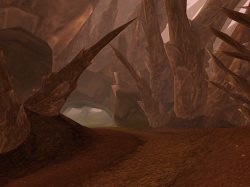
\includegraphics[width=\figwidth]{pics/12/37.png}
	\end{center}
\end{wrapfigure}
Sergeant Gravis had cleared us a beachhead, and those of us who hadn't gotten shot or cracked a rib on the way down widened it. 
That was our first chance to use the pulse weapons Tink and Fio had disguised for us on soft targets, and it was glorious. 
No heresy intended, but Tau carbines blow lasguns out of the water: 
they hit harder than a hot-shot, and reload easier too. 
We were dropping Nids and Orks left and right, and it was gratifying to see Sergeant Gravis stop and stare at us when he ran out of enemies.

The Space Marine didn't stop for long, or ask about our sexier-than-standard-issue weapons. 
Once he was sure we had the perimeter on lockdown, he switched to his Power Sword, and made his way towards the cluster of fallen spires that was occasionally illuminated by blasts of lightning. 
The Scout, who was perched similarly to Aimy and had stolen at least three of "her" kills, started following his boss by jumping from spire to spire. 


The official plan called for us to leave them to it, we were just supposed to secure a landing area for the shuttle and keep reinforcements out. 
We were doing far better than expected though, and Sarge started feeling all "I'm this Big Inquisition Guy who actually helps instead of just following orders," so he followed Gravis to lend a hand with the Zoanthrope, and Twitch tagged along for his own reasons. 
The rest of us were more than happy to stay put and keep shooting any Orks or Tyranids that wandered our way. 


Looking back, holding that perimeter was far too easy. 
There was never a concentrated attack on our position, just the occasional xenos who retreated in our direction or was checking out what all the plasma fire was coming from. 
We'd thought that the xenos were just keeping each other busy: 
the Tyranids weren't pouring in to reinforce their psychic artillery unit because the Orks were in the way. 
We didn't realize that something had gone wrong until Sergeant Gravis flew out the side of the rock pile.

\begin{wrapfigure}{O}{\figwidth}
	\begin{center}
		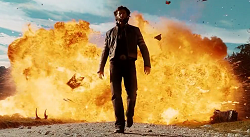
\includegraphics[width=\figwidth]{pics/12/38.png}
	\end{center}
\end{wrapfigure}
Well, not "flew" exactly, more like "was thrown". 
Something like a tonne and a half of Power-Armored Space Marine sailed through the air like a thing that is very bad at sailing, crashed through four of the smaller rock pillars, and barely activated its Grav-Chute in time to dodge a fatal collision with the larger fifth.

Doc tried to ask Sarge what the hell had just happened, but our fearless leader was busy screaming, swearing, and firing his pulse-carbine on full auto. 
When Doc tried again Twitch cut in, and in a slightly hysterical tone, told us that Sarge was busy right now. 
He suggested that anyone who wanted to live should get some cover between themselves and the rock pile; 
we didn't need telling twice.

Since we were keeping our heads as far down as was anatomically possible, and it turned out that Sarge was half-blind and Twitch wound up getting a nasty concussion, no one really saw what happened next. 
Luckily Spot recorded the whole thing.

A few seconds after Twitch's warning, he and Sarge came out of the rock pile at a dead sprint. 
They dove behind the first pillars they could find, and a split second later entire cluster of collapsed pillars exploded. 
Three green, glowing projectiles were propelled out of the hole Sarge and Twitch had exited, and splattered apart against the rock Aimy was perched on. 
One of them, or a random piece of debris, must have clipped Twitch's pillar too, because a sizable chunk broke off the top and nailed him on the helmet. 
He managed a dazed "Told you so" before collapsing.

In the aftermath, Doc ran over to check on Twitch and Sarge. 
The rest of us rest of us kept our eyes on the perimeter, except for Aimy. 
She descended from her gore-covered perch with a cry of "Oh god, it's everywhere. 
I think some got down my shirt. 
Tell me this isn't mashed Tyranids." Sarge blearily sat up, and told her not to worry: 
it was only mashed Orks. 
That did not improve Aimy's mood.

\begin{wrapfigure}{O}{\figwidth}
	\begin{center}
		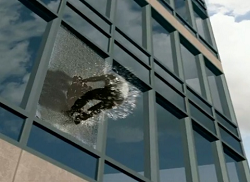
\includegraphics[width=\figwidth]{pics/12/39.png}
	\end{center}
\end{wrapfigure}
Sarge commed Gravis, verified that both the Marines had survived the blast, and made sure the shuttle was on its way to pick us back up. 
While we waited, and shot the occasional Ork or Nid that took an interest in us, Sarge explained what had happened inside the rock pile. 


Sarge had followed Gravis down a sort of tunnel that headed towards where the warp-lighting was coming from. 
The Space Marine had been sprinting ahead, and had obviously intended to rush the psyker with his Power Sword before it could notice and fry him with lightning. 
Sarge caught up just in time to see Gravis exit the tunnel and pull of the "close to melee range" part of the plan, but the xenos psyker hadn't been the frail ranged-support unit they'd expected. 
Instead, Sergeant Gravis wound up face to face with a big ol' psychic, not to mention psychotic and psychopathic, Ork.

To the Space Marine's credit, he hadn't hesitated at all. 
He'd waded right in and started chopping and stabbing while Sarge gave covering fire. 
Unfortunately, the Weirdboy had a bunch of bodyguards, and they bought him enough time to do some warpy stuff. 
Sarge said the moral of the story was: 
if a warp-energy infused Ork charges you with supernatural speed and a big glowy stick, it is a far better idea to dodge his swing than to try to block it with your Power Sword.

So when the Space Marine got knocked out of the park, Sarge'd decided it was time to leg it. 
He'd made liberal use of his flash grenades, and nearly ran into Twitch on his way out. 
Twitch had apparently been picking out the detonators for the detpacks he'd, without bothering to tell anyone, dropped all over the rock pile on his way down. 
Anyway, Sarge'd held the Weirdboy and his surviving minders off long enough for Twitch to sort out which button he wanted to press, and they got out of the pile a few seconds ahead of the explosion. 
The Orks hadn't, which was why Aimy was picking pieces of them off her armor.

\begin{wrapfigure}{O}{\figwidth}
	\begin{center}
		
\includegraphics[width=\figwidth]{pics/12/40.png}
	\end{center}
\end{wrapfigure}
Sergeant Gravis and his Scout rejoined us just as Sarge finished his story. 
Nubby, ever the diplomat, asked if their bug hunt had gone as well as our perimeter-securing had. 
Aimy and Tink snickered, but Sarge shut the three of them up: 
the two Marines didn't look like they were the mood for any bullshit.

Between the acid damage and the new set of dents and scratches, Gravis' armor was beginning to look rather ragged, and the Scout looked even worse. 
He'd apparently been trying to find a hole in the top of the pile to snipe through, and didn't have the same hard-wired response to a warning from Twitch that us guardsmen did. 
His stealth cloak was completely ruined, plus  there were at least two sizable holes in his carapace armour. 
He was still alive though, and rather rudely turned down Doc's offer to patch him up, so we figured he was fine and had learned an important lesson about warnings from demolitions troopers.

The stealth shuttle dropped out of the clouds above us, and we got back into the air without further incident. 
All of us more or less collapsed into the oversized seats. 
Despite the fact that we'd only been on the ground for about fifteen minutes, and only two us had been noticeably injured, we were exhausted. 
Our rest didn't last long though. 
Despite the perfectly reasonable suggestions some of us made concerning calling the mission off and pinning the blame on mister "73% certain it's an acceptable target," Sarge and Gravis both immediately started searching for another xenos psyker.

\begin{wrapfigure}{O}{\figwidth}
	\begin{center}
		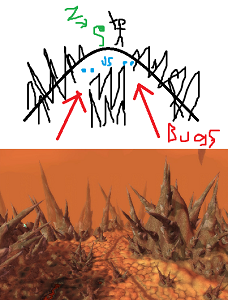
\includegraphics[width=\figwidth]{pics/12/41.png}
	\end{center}
\end{wrapfigure}
By the time we'd finished reloading, they'd found a slightly-less-rock-covered hilltop that was emitting lighting. 
 This time we had a clear view, and the lighting was obviously coming from a snakey-looking xenos which perfectly matched the images of Zoanthropes we'd seen. 
Gravis and his Scout did not find it amusing when Sarge asked for Twitch's opinion anyway. 
Luckily for for everyone's nerves, Twitch was too concussed to be smug, and simply agreed that the bug looked like a bug.

As our shuttle neared the hill we realized that this drop was going to be nastier than the last. 
This time, instead of a free-for-all, the hill was clearly in Tyranid hands/claws/whatever, and it looked fairly critical to the local battle with the greenskins. 
The Nids definitely weren't going to let us wipe out their artillery without a fight: 
they'd reinforce it as heavily as they could manage. 
Perimeter duty would not be another cakewalk, and if it took too long to subdue the psyker, we'd be up to our asses in bugs.

Sarge quickly split us into pairs, assigned us to the three main approaches to the hill, and convinced Twitch to share his mines with us. 
We'd clear the area, push out, then plant the mines and fall back towards the top if things got hairy. 
Before anything more complex could be put together, we reached the DZ.

Sergeant Gravis was the first one down again. 
He leaned out the rear hatch, sighted the Zoanthrope, and pretty much dropped right on top of the psyker. 
The rest of us followed as quickly and professionally as we could manage, none of us even had be pushed out of the shuttle by the Scout this time. 


\begin{wrapfigure}{O}{\figwidth}
	\begin{center}
		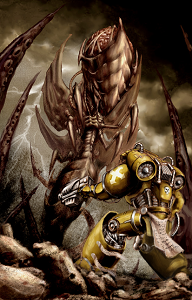
\includegraphics[width=\figwidth]{pics/12/42.png}
	\end{center}
\end{wrapfigure}
Every single one of us landed with our weapons firing. 
There were seven or eight Termagaunts keeping the Zoanthrope company, and only one of them was still alive when we hit the ground. 
Sarge finished that one off, and we all fanned out towards our assigned areas. 


We moved fast, motivated by a desire to get our chokepoints set up before reinforcements arrived, and to get something solid between us and Gravis' fight with the Zoanthrope. 
Honestly we hadn't taken the Space Marine too seriously up to that point. 
I mean we respected him and found him daunting as hell, but his combat performance in the last drop hadn't been up to the stories you hear about Space Marines. 
His fight with the Tyranid Psyker though, that was something to tell your grandkids about. 


In the few seconds we saw him fighting before we got under cover, Sergeant Gravis baited out and dodged three massive lightning bolts, scored twice as many hits on the Xenos' shield bubble, and generally moved with more speed and grace than should have been possible. 
Abstractly we'd known that the Emperor's Scythes Chapter were the best experts available when it came to fighting Tyranids, but watching Gravis play that Zoanthrope like a fiddle really drove it home. 
We all would have stopped to spectate, if the Zoanthropes misses weren't blowing the rocks near us into red-hot shrapnel that is. 


Anyway, we all got the hell off that hilltop and into position. 
Spot stayed up high, and gave us a good view of the incoming reinforcements as we set our mines and found the best lines of fire. 
We all finished our preparations just in time, and started mowing down the first wave of Tyranids as they climbed the hill.
\begin{wrapfigure}{O}{\figwidth}
	\begin{center}
		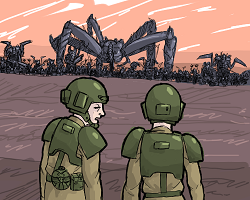
\includegraphics[width=\figwidth]{pics/12/43.png}
	\end{center}
\end{wrapfigure}
That first wave was nothing but the Gaunts, both varieties, that had been near the hill. 
Thanks to the wonderful nature of chokepoints, not to mention good firing positions and techno-heretically awesome weapons, we were able to kill them all before they managed to shoot or claw us. 
That's not to say that we actually killed ALL of the Tyranids, Nids don't tend to run out of bodies to throw at a problem, but we did convince them to rethink their strategy. 
Once the choke points were too, well, choked with their bodies for any more to get past, the Gaunts broke off to wait for heavier reinforcements.

Now, we'd been in this sort of fight with Nids before. 
Back when we were actually in the Guard we'd fought a memorable, and debatably successful, defensive battle against the bugs. 
So, we knew what would almost certainly come next: 
Warriors, possibly with Ravener or Gargoyle support. 
On our respective sides of the hill, Aimy, Nubby, and Tink all moved to elevated positions and helped Spot watch for the higher lifeforms. 
Meanwhile, those of us still on the ground made sure the mines and our next positions were ready, and Sarge checked in with Gravis and his Scout. 
The Marines were still working on wearing down the Zoanthrope's shields without killing it, and asked us not to distract them again. 
We all made some rather unkind comments at that last part, but refrained from transmitting any of them.

Spot the Wonder Drone tagged the second wave on its way in, and as we'd guessed, there were some Warriors directing the charge from behind the initial meatshield. 
The Guard has a Standard Combat Doctrine for pretty much every situation. 
While most of these are not very individual-Guardsman-friendly, the one for that sort of attack is a good'un, so for once we did things by the book. 
Admittedly said book is rather short, but that just means it's easy to remember. 
The three of us that had moved into sniper positions held our fire, and prepared to "Shoot the Big One First."

\begin{wrapfigure}{O}{\figwidth}
	\begin{center}
		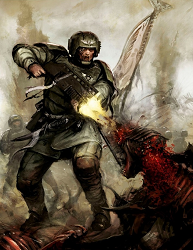
\includegraphics[width=\figwidth]{pics/12/44.png}
	\end{center}
\end{wrapfigure}
On Doc and Tink's flank, an overcharged, Tau-laser-thingy-guided plasma bolt turned their Warrior into chunky salsa. 
Over on Aimy and Twitch's, a precision headshot from our actually-quite-talented markswoman took out theirs. 
With the synapse creatures dead, the Gaunts lost cohesion and both pairs of guardsmen easily mowed them down. 
Unfortunately the sniper on the third flank was Nubby, who didn't have Tink's anti-armor weapon or Aimy's accuracy.

A very angry, if rather burnt and bloody, Tyranid Warrior immediately returned fire with one of those big bee-gun things, pinning Nubby down on his sniper perch. 
Sarge tried to hold off the incoming wave himself, making heavy use of his grenades and the chokepoint, but it quickly became apparent that it wasn't going to work. 
Sarge commed the rest of us and, over Nubby's shrill screaming, asked if anyone could give him support before he had to blow his mines and relocate.

The rest of us were still rather busy with our mop-ups, and reinforcing Sarge meant crossing the Zoanthrope infested hilltop, so we all declined. 
It seemed like Sarge was going to have to give up his flank's safety margin, and he was getting ready blow his mines and pull Nubby out, when the Scout Marine told him to hold a little longer. 
Sarge managed it. 
He wound up having to use his boots to keep an especially persistent Gaunt off while he reloaded, and his armour and beefiness barely saved him from a few fleshborer hits, but he managed it. 
Right as things were getting downright dire, the Warrior and several nearby Gaunts went down to an amazing display of precision shooting.

Nubby finally got his ass out of cover, and helped Sarge turn the tide back around as the Scout returned to the Zoanthrope fight. 
Things were looking pretty good, even if we could see the third wave mustering near the bottom of the hill. 
Good changed to Great when we heard Gravis say the Zoanthrope's shield was almost down. 


And then everything went to shit.

\begin{wrapfigure}{O}{\figwidth}
	\begin{center}
		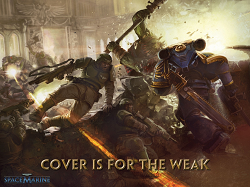
\includegraphics[width=\figwidth]{pics/12/45.png}
	\end{center}
\end{wrapfigure}
Looking back, it's not that hard to spot the exact moment when the shitting of the everything occurred. 
Actually it wasn't that hard to spot at the time either, within twenty seconds of it happening we knew what had gone wrong and why, but it took a bit longer for all the horrible results of that one screwup to manifest.

Anyway, what started that whole horrible shit-show was a simple communications failure at a rather hectic moment. 
The third wave of Tyranids was coming in, and we were busy shooting them and getting ready to blow our mines and fall back. 
Up on top of the hill, Sergeant Gravis had the Zoanthrope on the ropes and was ordering his Scout to get ready to tranq it. 
The Scout Marine had just returned from helping Sarge, and was perched on one of the pointy pillars on top of the hill. 
As the Scout got the tranq ready and lined up what must have been a rather tricky shot, he spotted something and commed us. 
His EXACT words were: 
"Interrogator, Incoming Tyranid Assault Flier, North Side."

Now let's do an experiment. 
First, go out and find fifty thousand Guardsmen. 
Actually, go out and get a hundred, it's not like Guardsmen hard to find. 
Hell, we're literally the largest organized fighting force in the galaxy. 
Which, come to think of it, means that the definition of a standard response to ANYTHING, is what WE do, not what a few bloody crazies stomping around in power armor and getting eaten by bugs…

ANYWAY, ask any of these Guardsmen what they'll do when someone warns them hostile air units are incoming. 
Nothing else, no details or orders, just Hostile Air Incoming. 
You know what they'll say? 
It'll be the same regardless of regiment, specialization, rank, or anything. 


Every. 
Single. 
One of Them. 
Will tell you the same thing: 
THEY WILL GET THE HELL INTO COVER.

Apparently the Emperor's Scythe's Chapter of The Space Marines aren't on the same page as the rest of us though. 
Or at least that Scout Marine wasn't.

\begin{wrapfigure}{O}{\figwidth}
	\begin{center}
		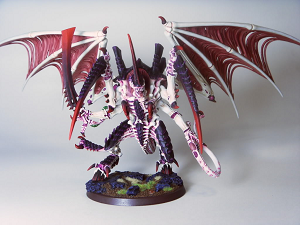
\includegraphics[width=\figwidth]{pics/12/46.png}
	\end{center}
\end{wrapfigure}
I mean if he'd just been a little more clear... 
If he'd added just a few more bloody words, like: 
"TAKE IT OUT" or "COVER ME", or even if he'd just shortened it to: 
"INCOMING ASSAULT" we would've understood… 

But no, he told us there was a Flier Incoming, and stood there with his ass hanging out, wrongly believing that we'd shoot it down while he lined up his shot on the Zoanthrope.

Nubby was the first one to notice the impending disaster. 
Well actually he just saw the Scout standing there, and told Sarge that the "stupid bastid's gonna get 'is arse shot off." Sarge stared for a second, then peeked out of cover and saw what sort of flier was incoming. 
Everything started to click together, the incoming Tyranid wasn't some dedicated air biofom designed to strafe or bomb ground targets. 
It was biggest, meanest melee monstrosity in the swarm, or at least the biggest one that was was still capable of flight. 


It was a Flyrant. 
A Winged Hive Tyrant. 
The Tyranid equivalent of a Lord General crossed with a Main Battle Tank and with some wings strapped on for good measure. 
It was big, pissed, and coming right at the only member of our team that was standing out in the open.

Unfortunately Sarge was just a little too late. 
By the time he'd started shouting his warning, nearly five tonnes of flying Tyranid hit the Scout Marine in the back. 


You know how in cartoons a bus or train hits someone and they'll just sort of vanish? 
It was exactly like that, right down to how the poor bastard's sniper rifle was left pinwheeling in the air for a second.

In the aftermath three things became apparent: 
the Scout had not gotten his shot off, the psychically exhausted Zoanthrope was doing a runner, and Gravis had bigger problems than chasing it. 
The Space Marine told us that the Zoanthrope was fleeing towards Sarge, asked us to catch it, and then started shouting about some place called Sotha. 
A second later the Tyrant let out scream that shook the entire hilltop.

\begin{wrapfigure}{O}{\figwidth}
	\begin{center}
		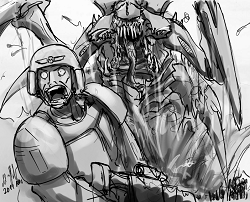
\includegraphics[width=\figwidth]{pics/12/47.png}
	\end{center}
\end{wrapfigure}
The situation was bad, but it was also, thank the Emperor, relatively simple. 
We had a perimeter to maintain, a Hive Tyrant to survive, and a Zoanthrope to catch. 
Sarge started bellowing out orders and the rest of us scrambled to follow them.

Since we still had all of our mines in place, the perimeter was actually the least pressing issue. 
Sarge's first order was to fall back towards the top of the hill, and let the explosives hold off the smaller Tyranids for a while. 
Sarge then told us he was going after the Zoanthrope, and sent Nubby to get the Scout's tranq-loaded sniper rifle. 


For the rest of us, Sarge's final orders were a little more… freeform. 
Tink was to get his drone on the Hive Tyrant, and the rest of us were told to "HANDLE IT." Seriously, that was his entire master plan. 


\greentext{>By the Emperor! There's a bloody HIVE TYRANT inside our perimeter, it's killed one Space Marine and, as soon as it finishes off the other, it'll kill us all. What should we do sir? }

\greentext{>"HANDLE IT"}


He never managed to live that one down. 


The ridiculousness of that order aside, it's not like we actually needed one. 
Each of us knew that the only way we'd live through this was if the Tyrant was dead, forced to retreat, or kept distracted long enough for us to call and board the shuttle. 
All three of these possible solutions could be accomplished in the same way: 
by shooting the big bug and running away if it chased us. 
Some variations and improv could be thrown in as things progressed, but Shoot and Run was really the core strategy. 
Even the Space Marine was doing it, though it was more Stab and Run in his case.

\begin{wrapfigure}{O}{\figwidth}
	\begin{center}
		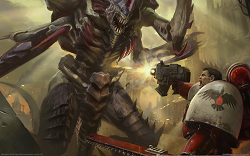
\includegraphics[width=\figwidth]{pics/12/48.png}
	\end{center}
\end{wrapfigure}
The first of us to actually see the Hive Tyrant up close were Aimy and Twitch. 
As they ran up towards the hilltop, Sergeant Gravis started coming down in these big graceful leaps made possible by his Grav-Chute. 
Valiant Heroes of the Imperium that both of them were, they immediately scrambled to find hiding places. 
As the massive Tyranid charged down after Gravis, both of them held their fire, not to mention their breaths, and observed what they could. 


The Flyrant was, of course, a winged bipedal bug that stood six meters tall and was made of distilled murder and hate, but it also had a few important distinguishing points. 
It had four arms, well three-ish after Gravis had gotten its attention. 
The top one-and-a-half ended in the usual Tyranid talons, the bottom pair held a massive bonesword and one of those freaky sentient whip things. 
Each of those weapons was capable of messily killing any poor guardsman that got in close, but none of them had real range. 
That was a very good thing for us, not so much for Gravis though.

Speaking of Sergeant Gravis, he was coming down the hill fast, but the Flyrant was gaining and he didn't have much room left to run before he hit Twitch and Aimy's minefield. 
Right as it looked like he was going to try jumping over it and then wading through the incoming wave of Nids, he suddenly reversed direction. 


All three of the Flyrant's attacks missed the Space Marine as, with more speed and agility than anyone wearing the equivalent of a light-tank should have, he dodged between the beast's legs. 
It was impressive as hell, especially the part where he got in a whack with his Power Sword on his way through. 
Both Aimy and Twitch watched appreciatively; 
until they realized the Flyrant wasn't going to be able to stop.

The four-point-nine tonne Tyranid flailed it's wings in a mad attempt to get airborne, completely failed to do so, and plowed through over a dozen AP mines. 
Twitch and Aimy barely made it into new cover in time.
\begin{wrapfigure}{O}{\figwidth}
	\begin{center}
		
\includegraphics[width=\figwidth]{pics/12/49.png}
	\end{center}
\end{wrapfigure}
Of course it takes more than a few AP mines to kill a Hive Tyrant. 
Aside from shredding its wings, all they really seemed to do was piss it off. 
The Tyrant let out another of its piercing shrieks as it reversed direction, and started pelting back up the hill after Gravis. 
Twitch and Aimy watched it go, then realized they had a bit of a problem, namely that there was no longer much of a minefield between them and the wave of smaller Tyranids.

The debate over what to do consisted of Aimy and Twitch pointing in opposite directions, yelling "HANDLE IT" at eachother, then splitting up. 
Twitch ran around dropping the last of his mines and spraying fire at the incoming Gaunts. 
Aimy sprinted up the hill after Gravis and the Flyrant, hip-firing her pulse rifle at the massive target until it crested the hill and she lost line of sight. 


When Aimy reached the top of the hill, she found Sergeant Gravis carefully circling around the enraged Flyrant while Doc and Tink shot it. 
Like the other two Guardsmen, she sighted on the Tau marker-thingy Spot was projecting on the Tyranid and poured out as much fire as she could. 
It was beginning to look like the three of them would be able to wear the creature down, then Gravis botched one of his dodges.

The Space Marine had to choose between trying to block the Flyrant's bonesword or dying a horrible death, and reluctantly chose the former. 
For the second time that day, he flew through the air with all the grace and aerodynamics of a thrown brick.

Sergeant Gravis ricocheted off one of the stone spires encircling the hilltop, briefly tumbled upwards, then crashed into the dirt directly behind Doc and Tink. 
He was a tough bastard though: 
within a second of his landing started moving again. 
Both the Space Marine and his armor groaned as he struggled to get back on his feet.

The Flyrant let out yet another roar, sighted on the recovering Space Marine, and charged.
\begin{wrapfigure}{O}{\figwidth}
	\begin{center}
		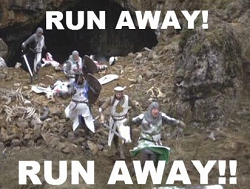
\includegraphics[width=\figwidth]{pics/12/50.png}
	\end{center}
\end{wrapfigure}
Now, in your normal Commissariat Approved Uplifting Story of Heroism, this is where the two Stalwart Guardsmen would've stood their ground and laid down their lives to buy the wounded Space Marine time to recover. 
Then, right after the Guardsmen had finished valiantly sacrificing themselves, he would've magically gotten better and killed the vile Xenos. 
Oh, and then all the Orks and Tyranids on the planet would've died, and it the whole place would've turned into a garden world that paid all it's tithes on time, and there'd be statues of the heroic dead Guardsmen everywhere…

The warp take those stories, and whoever keeps writing them, and the whole Commissariat for that matter. 
Ever notice how it's always some Guardsman and never the Commissar who dies horribly in the Emperor's name? 
Anyway, Doc and Tink took one look at the charging Flyrant, and ran for it.

Okay, I realize that sounds bad, but it's not like they ran down the hill and left Gravis to die. 
They kept firing and ran perpendicularly along the top of the hill in, and I quote the official report here, "An attempt to draw the Hive Tyrant's attention away from its target." Anyway, it's not like they would've accomplished anything by standing there, and there was no way either of them could've carried a fully armored Space Marine to safety. 
My point is that what happened next was NOT Doc's, Tink's, or anyone else's fault, and I'll have you know that the tribunal of senior Ordos Xenos Inquisitors who reviewed Spot's footage agreed with that assessment. 
Well, two thirds of the Tribunal anyway.

So while three of us poured a hell of a lot of plasma into the Flyrant, it closed to melee range with Sergeant Gravis. 
He parried the beast's whip-thing, sidestepped a strike from its single remaining talon, then did that trick where he dodged through its legs again. 
Whereupon the Flyrant turned, brought its bonesword around at mid-chest-level, and cut Sergeant Gravis in half.
\begin{wrapfigure}{O}{\figwidth}
	\begin{center}
		\includegraphics[width=\figwidth]{pics/12/51.png}
	\end{center}
\end{wrapfigure}
Twitch finished laying his replacement minefield and arrived on the hilltop right then, as did Sarge and Nubby, who were lugging the tranqed Zoanthrope between them. 
Their part of what could be generously called "the Plan" hadn't involved anything as terrifying as the Flyrant, but it hadn't been a cakewalk either. 


Sarge had managed to sight the fleeing Zoanthrope as it came down the hill towards him. 
It turned out that even when too exhausted to keep itself hovering, the psyker bugs are capable of wriggling along the ground at a surprisingly high speed. 
While Nubby hunted down the Scout's dropped rifle and its tranq round, Sarge chased the Zoanthrope back and forth between the rocks, dodging the occasional weak lighting bolt and stray fleshborer round as he did so. 
Eventually he corned the beastie between two spires right as Nubby arrived with the comically oversized Astartes Pattern Sniper Rifle.

Since it quickly became apparent that Nubby was completely incapable of aiming the oversized rifle, and the Zoanthrope was still squirming around a lot, Sarge decided to take the shot himself. 
The second he was distracted the bug tried to escape again, and Sarge wound up tackling the thing and trying to pin it to the ground. 
It was like wrestling a cross between a greased pig, a giant snake, and an uninsulated power conduit. 


In the end he collected a few scratches, a nasty bite wound, and a whole lot of electrical burns before Nubby just dragged the rifle over and jammed it into the Zoanthrope's under-belly. 
Then they hauled the surprisingly long and heavy xenos up to the hilltop, pausing to chuck a few grenades at the incoming wave of Nid reinforcements on the way, and got there just in time to see Gravis' bisection.

There was a brief silence, which was punctuated by two meaty thuds and Nubby's nasal voice.

\greentext{>'Oly shit... fink ees gonna be okay?}


Then the Flyrant roared again and all six of us open fire.
\begin{wrapfigure}{O}{\figwidth}
	\begin{center}
		\includegraphics[width=\figwidth]{pics/12/52.png}
	\end{center}
\end{wrapfigure}
Spot was projecting its Tau laser-thingy on the middle of the Flyrant's torso, and we all just sighted our weapons on it and held the triggers down. 
Looking back it's hard to say whether it was sheer weight of fire, or if the big bastard was just running out energy, but it's charge towards us was much slower than its earlier ones had been.

Every single one of us got an entire magazine's worth of shots out before the flyrant was a third of the way to Sarge and Nubby. 
It never made it to two thirds, there was a sort of squelchy pop as it's torso armor gave way, and the beast stumbled. 
It sort of huddled there, trying to protect its wounded chest, and sending out a screech that was echoed by the smaller Tyranids climbing the hill. 
From the sound of it, they were finally getting passed our minefields, and would be arriving in seconds.

None of us went to hold off the incoming reinforcements though. 
The Flyrant was the very definition of "The big one", and we were going to shoot it first. 
Spot redirected it's markerlight to the xenos' head.

Not that we actually needed the fancy tau flashlight though: 
even if the Flyrant's head was a relatively small target, it was a stationary one now. 
Every shot we fired hit, and within seconds our massed plasma fire either punched through the Tyranid's head amour, or cooked the thing's brains to boiling point. 
It's head exploded like a particularly disgusting grenade, and a psychic pressure that none of us had even noticed was released. 
All around the hilltop the incoming Tyranids broke and fled as quickly as they could, and the Zoanthrope twitched a little where Sarge and Nubby had dropped it.

Let me tell you, we'd escaped near certain death before, but the relief we all felt on that barren hilltop was greatest in our lives. 
Every one of us just stood there and basked in the sheer joy of still being alive. 


Then Tink spoiled it by asking if Gravis had called the shuttle before he died.
\begin{wrapfigure}{O}{\figwidth}
	\begin{center}
		\includegraphics[width=\figwidth]{pics/12/53.png}
	\end{center}
\end{wrapfigure}
Tink's question was followed by the sound of a few thousand Orks Waaagh-ing, and it occurred to us that we'd probably just killed the creature that'd been holding the Tyranid defense of these hills together. 
I doubt anyone in the history of the Imperium has ever gone from ecstatic relief to blind panic as quickly as we did.

Sarge started wildly flipping through comm channels, Twitch ran around deploying the last of his explosives, Aimy screamed at Tink for not remembering sooner, and Tink called Aimy a skunk-haired super-bitch. 
The odd men out were Doc, who had gone right past panic to depression, and Nubby, who defaulted to some very basic instincts when overwhelmed. 
While everyone else was busy screaming, shouting, mining, and crying, Nubby went to get himself a shiny, not-quite-new Power Sword.

The cretinous little vulture found the Sword still in Gravis' hand, which didn't deter him even slightly. 
He firmly planted a boot on the Marine's arm and started prying at the power-armored fist. 
As Nubby levered off the smallest of the Marine's fingers, two practically reflexive actions occurred. 
First Gravis shook Nubby's grip off and tightened his fingers on his Power Sword. 
Second, Nubby automatically responded by drawing his combat knife and preparing to give the Emperor's Peace, thereby settling any silly little ownership disputes. 


It was immensely lucky for all of us that Gravis' ceramite helmet was still sealed, since it made trying to slit his throat long and noisy process. 
Doc noticed Nubby going at the Space Marine's armored neck like an incompetent lumberjack, realized what it implied, and bodychecked Nubby off the not-quite-dead Sergeant Gravis. 
Our brilliant medic then stood there, with his medkit open, panicking and trying to figure out how to treat the mother of all chest wounds.
\begin{wrapfigure}{O}{\figwidth}
	\begin{center}
		\includegraphics[width=\figwidth]{pics/12/54.png}
	\end{center}
\end{wrapfigure}
The commotion caught Sarge's attention in turn, and he abandoned his fruitless attempts to contact the shuttle by randomly trying comm channels. 
Sarge's first question wasn't if Doc was sure Gravis was still alive, or how that was even possible, it was whether the Space Marine was capable of calling for evac. 
Doc gibbered, and pointed out that Gravis' lungs had been cut in half and he could actually see INSIDE them. 
Sarge took that as a no, but noticed Nubby's knife stuck between Gravis' helmet and gorget. 
Without waiting for a medical opinion, he seized the knife and twisted it with all his beefy-noncom strength. 


Later it was explained to Sarge, but not Nubby, that the latches on Mark VII Power Armor helmets don't actually lock, and he could've just flipped them open. 
At the time though, Sarge was too busy to waste time thinking, and just tore apart several million thrones worth of data-relays and void-seals. 
When the helmet finally came off, with a tear and a snap rather than a little pop, Sarge ran over to where Aimy was beating seven kinds of shit out of Tink. 
He ended their friendly little argument over who "the real bitch" was by grabbing the back of Aimy's Ork-stained armor, and unceremoniously chucking her in Twitch's direction. 
Sarge then dragged Tink to his feet, thrust Gravis' helmet into the techie's hands, and screamed at him to make the vox work.

Tink stared at the helmet for a second, realized he had absolutely no idea how it worked, and wisely decided to try the obvious thing first. 
Which is to say, he put the helmet on his head and hesitantly asked if the thing was on. 
He was nearly deafened by the shuttle pilot's screaming request to know what the hell was going on and what had happened to Sergeant Gravis. 
Tink decided that Sarge could answer that question, handed the helmet over with a smug little line about being able to fix anything, and went to see if Doc had anything for a broken nose.

He immediately regretted that decision.
\begin{wrapfigure}{O}{\figwidth}
	\begin{center}
		\includegraphics[width=\figwidth]{pics/12/55.png}
	\end{center}
\end{wrapfigure}
So Sarge was wearing the helmet and explaining things to the Shuttle pilot, Twitch was being Twitch, and since it looked like we actually wouldn't all be left stranded in the middle of an army of Orks, both Nubby and Aimy decided it was time to take a breather. 
They sat on the tranqued Zoanthrope, shared a pack of Lho sticks, and enjoyed the sight of Doc freaking the hell out and shaking Tink like a terrier with a rat.

\greentext{>OH GOD WHAT DO I DO?}


I dunno, fix him or something, STOP SHAKING ME

\greentext{>HOW TINK? How do you fix BEING CUT IN HALF? He shouldn't even be alive, I don't know what's going on here, I don't know how Space Marines work! What if touching him makes it stop working? WHAT DO I DO?}


Umm umm umm…. 
do that Space Marine thing!

\greentext{>WHAT THING?}


Harvest his geneseed!

\greentext{>His what now?}


His geneseed! 
It's like this seed thing that Space Marines have, if you pull it out before a Marine dies you can plant it in a servitor and he grows back from it. 


\greentext{>Really?}


Yeah, they had this whole thing in the last season where Brother-Captain Markus the Cooperator fell in battle, and the fire-warrior rescue team had to-

\greentext{>Wait, you mean in your Tau vids? You're basing this off heretical cartoons?}


THEY'RE NOT CARTOONS,THEY'RE NOT HERETICAL, AND DO YOU HAVE ANYTHING BETTER?

\greentext{>Shit shit shit shit shit… okay what's this "geneseed" look like and where does he keep it?}


Ummm they had to censor the part where they cut it out, but I think it was like a second heart thing, and it was all green and stuff.

\greentext{>Heart thing, so like in his chest?}


Yea, right in the middle.

\greentext{>Okay, in the chest… Upper chest or lower chest?}


Umm

\greentext{>UPPER CHEST OR LOWER CHEST? If I'm going to be digging around inside him looking for something green, I at least need to know which end to dig around in!}


I don't know, why doncha go check on the Scout?

\begin{wrapfigure}{O}{\figwidth}
	\begin{center}
		\includegraphics[width=\figwidth]{pics/12/56.png}
	\end{center}
\end{wrapfigure}
The Scout Marine was pinned to the hilltop's ground a few dozen meters away from where he'd been perching when the Flyrant hit him. 
I'm using "pinned" quite literally here, he was face down with a Tyranid talon the size of a beefy telephone pole through his back. 
The talon ended in a very neat cut that matched the stump the Flyrant had, which probably explained how Gravis had gotten its attention.

Unlike Gravis, there wasn't much confusion over whether the Scout was dead: 
he'd started to go runny. 
It's not like all of him was melting, just a sort of expanding area around where he'd been speared. 
Said area included both the upper and lower chest though. 
In the name of medical science, Doc poked at the mushy corpse with a probe, then jumped backwards with a girly shout when it started to hiss and melt too.

\greentext{>Emperor...  I swear he wasn't doing that earlier. Is this like a Space Marine thing? Do they melt when they die?}


Ewww, don't think so, would make it hard to re-use the armor. 
Bethcha it's a Nid thing, does yer Big Book-o-Pseudoscientific Medical Bullshit have a section on Tyrant bioweapons?

\greentext{>Umm, umm, umm, Tyranid, tyrant, umm, umm, bonesword, scything talon, TOXIN SACS!}


Huh, neat, what's it say?

\greentext{>If in fully stocked field hospital… laboratorium... quarantine… here! Battlefield instructions! "Smear area with counterseptic, administer oral De-Tox, scan and apply indicated Toxin Wands, give Plasma, pray to the Emperor." I CAN DO ALL OF THOSE!}


Wait, like plasma from a gun or a bag? 
And what about the geneseed though? 


\greentext{>Screw your geneseed, if we can keep him from melting until the shuttle arrives we can ask the pilot. Now take these and go to his bottom half}


These are pills Doc, how do I give a pair of legs pills?

\greentext{>HOW DO YOU THINK?}


Oh god, I am NOT qualified for this…

\greentext{>Well neither am I, now DO IT.}


\begin{wrapfigure}{O}{\figwidth}
	\begin{center}
		\includegraphics[width=\figwidth]{pics/12/57.png}
	\end{center}
\end{wrapfigure}
Doc's panicked medical treatments were of rather dubious usefulness, especially the part where he fed a De-tox tab to the nearly-dead Space Marine. 
That stuff is nearly enough to kill you on its own, and it made the big guy flail around and spurt some nasty stuff out the end of his torso, which at least it proved he was alive despite the whole not-really-breathing thing. 
Also, Doc put more fluid back in, and sealed off most of the leaky, exposed torso area, so it was probably a net gain for Gravis.

We all watched him running around and yelling at Tink, who was stuck with the literal ass-end of the job, while the sound of the oncoming Orks grew steadily louder. 
It came as an immense relief when the shuttle dropped out of the clouds, and you better believe we were lined up and ready to board before it'd hit the ground. 
The pilot wasn't exactly on the same page as the rest of us though: 
he didn't stay in his seat and keep the engines spun up, instead he was standing at the rear hatch when it opened.

None of us had actually seen the Pilot on our flight in, and that first meeting was rather unpleasant. 
He was a Scout Marine and looked nearly identical to the other guy, except for not being impaled and dissolving. 
He was also considerably worse at the whole Stoicism thing. 
The Pilot stood in our way and demanded to know what had happened to Sergeant Gravis and Rubram, which was sort of awkward since none of us had actually bothered to learn the dead Scout Marine's name. 
Anyway, the Pilot did not take his sergeant's bisection well, and nearly went berserk when he saw his buddy's rifle sticking out of Nubby's pack.

The outermost mines were going off at this point, and none of us wanted to die on landing pad, so Sarge acted rather cruelly. 
He yanked the "le-gi'-a-men' ba'lefiel' salvage" out of Nubby's pack, thrust it in the Pilot's arms, said the Scout had wanted him to have it, and then pointed out that his boss was GOING TO DIE IF WE DON'T TAKE OFF RIGHT NOW.

\begin{wrapfigure}{O}{\figwidth}
	\begin{center}
		\includegraphics[width=\figwidth]{pics/12/58.png}
	\end{center}
\end{wrapfigure}
We didn't have any problem securing the Zoanthrope for takeoff, the snakey xenos was still completely out of it and fit right into one of the oversized seats, Gravis was a bit of a problem though. 
Doc wound up strapping him UPSIDE DOWN in one of the seats, supposedly because it let him tighten the crash harness and would keep everything from falling out if the bandage gave way. 
None of us knew enough to argue, so we went with the same gross-end-up theory for his lower half, which was put into the seat next to him. 
During the strapping-in process Gravis' sword, bolter, and other little weapons and gadgets disappeared into Nubby's backpack. 
Thankfully the Pilot was too busy taking off and dodging small-arms fire from the incoming Orks to see any of this.

After we were out of the Orks' range, our ascent out of the atmosphere went comfortably enough. 
Sarge sat in the relative peacefulness and inspected us troops. 
In addition to his ample supply of lacerations and electrical burns, we'd collected a concussion, a fairly nasty leg wound, a broken nose, some cracked ribs, nearly a dozen minor fleshborer hits, and an Ork-juice marinade. 
We were all still alive though, and we had Oak's Zoanthrope too, so all-in-all, we called it a win.

Sure, our Space Marines had taken one hell of a beating, but we'd completed our objective and horrible sacrifices in the name of victory are what Space Marines are all about. 
 I mean we'd been attacked by a bloody Hive Tyrant, and two Marines for a Tyrant is a pretty good trade. 
Anyway, it was beginning to look like Gravis might just survive long enough to get him to a real medicae. 
So yea, totally a win.

We were in the middle of congratulating ourselves and speculating on if Gravis would be put in a Dreadnaught when three things happened. 
First the Zoanthrope started twitching, then Gravis' armor started beeping and his lower half began to smoke, and finally the helmet in Sarge's lap started talking.
\begin{wrapfigure}{O}{\figwidth}
	\begin{center}
		\includegraphics[width=\figwidth]{pics/12/59.png}
	\end{center}
\end{wrapfigure}
So no shit there we were, sneaking across a warzone with a slowly awakening Tyranid psyker and a quickly dying Space Marine, when Sergeant Rebus called for his evac. 
If you actually needed proof that the entire purpose of the universe is to shit on poor hardworking Guardsmen, it'd be damned hard to find something better than that timing right there. 


I mean, just to remind you, this wasn't some simple pickup from a combat zone he needed. 
No no no no no, he needed us to sneak back into boarding range of a Tyranid Hive ship, which was still being assaulted by a few million Ork Fightas, to pick him up before the high-yield Vortex Bomb he'd just planted, went off. 


You could say that we weren't the ones doing the actual sneaking, and that we'd been safely through it before, without the armed Vortex Bomb of course. 
But this time it would be a race against the Zoanthrope waking up and Sergeant Gravis melting. 
Every man has their limit, and this was well beyond ours. 
Before the Pilot could respond, Sarge put on Gravis' helmet, and calmly, clearly told the Space Marine to Wait His Damned Turn. 


All of us, except for Doc who was rather busy, cheered. 
Sergeant Rebus and the Pilot were less enthusiastic.

The argument that followed included accusations of cowardice, the Pilot coming out of the cockpit with a Bolter and threatening to kill either us or the Zoanthrope, and Sarge telling one of the Emperor's Angels of Death to "Shut up and soldier, Soldier." In the end, a combination of devotion to the mission and desire to save HIS sergeant won the Pilot to our side. 
Sergeant Rebus was instructed to delay the bomb's detonation and hold out until we were dropped off and a return trip could be made. 
The conversation ended with Rebus bitterly complaining that dying waiting for evac was an end worthy of a Guardsman. 
Sarge responded by telling him that Holding The Line wasn't that hard: 
after all, us Guardsmen did it all the time.
\begin{wrapfigure}{O}{\figwidth}
	\begin{center}
		\includegraphics[width=\figwidth]{pics/12/60.png}
	\end{center}
\end{wrapfigure}
Now it might sound like we callously doomed a team of valiant Space Marines to their deaths, but we really weren't delaying their extraction THAT long: 
the Marines had prepared for this type of situation when they'd adjusted their mission plan to account for only having one shuttle. 
The Occurrence Border had followed our stealthy little vessel into the system as quietly as it could, and was now close enough that it'd be a matter of minutes, not hours, to reach it. 
Of course, being that close meant there was a significant risk of detection, and the Occurrence Border did not have any real way to hold off and attack by the Orks or the Nids. 
Back at the briefing Rebus had claimed it was an acceptable risk though, which goes to show you what a bloody tactical genius he was.

Okay, maybe that's a little unfair. 
Having the ship closer turned out to be very good for him, and it's not like he could've foreseen that we'd capture the Zoanthrope, but forget to bring along the second dose of that special psyk-tranquilizer stuff. 
Though if he's spared the blame, then that means Gravis and his Scout deserve a little for not taking the excessively simple precaution of leaving a few spare doses in the shuttle. 


I mean we were going into extremely hostile territory, why was the Scout carrying ALL the tranqs, and why hadn't either of them told us a second dose would be needed? 
Is Tyranid wrangling some super-secret Emperor's-Scythes-only technique? 
Or did they think that there was no way that we'd survive and continue the mission if they didn't? 
Well, actually that one is completely understandable, arrogant as all hell, but understandable.

I'm getting ahead of myself though: 
the Zoanthrope was a problem later. 
At the time our big concern was that half of Gravis was dying and the other half was violently decomposing.
\begin{wrapfigure}{O}{\figwidth}
	\begin{center}
		\includegraphics[width=\figwidth]{pics/12/61.png}
	\end{center}
\end{wrapfigure}
Once again the task was divided between Doc and Tink. 
This time Doc was much calmer, and his response was surprisingly reasonable and professional. 
He fussed around the upside-down Space Marine torso with his medical scanner and Tox Wands, and shouted questions about Astartes biology and Power Armor automated medicae systems at the Pilot. 
There was some rather confusing talk about Illicit Kidneys, Biomedical Cogitators, and Cellular Regenerator reservoirs, which the rest of us ignored, because Tink's part of the job was a complete shitshow.

Whatever was on the Flyrant's sword, when it got going, it REALLY got going: 
Gravis' lower half went from fine to melting from the wound down, in mere seconds. 
It's hard to say whether Tink's response was best or worst one available, but it was certainly the most disgusting. 
In an effort to slow down the process, he unbuckled the power-armored legs, and flipped them upside down. 
The smoldering bandage immediately gave way and dumped a horrible combination of meat-juice, xenos toxins, and extremely powerful acid onto the seat. 
The smell was beyond vile, and all of us had to put on our rebreathers just to stay conscious, which was lucky considering how many airborne toxins were found in that shuttle when we landed.

So after the spillage started dissolving the seat, the rest of us became very interested in helping Tink. 
Of course none of us knew jack about biochemistry, so we were only able to offer what might be called Mechanical Solutions to the acid problem, and most of those suggestions were absolutely terrible. 
In the end we settled on the traditional Occurrence Border technique of shoving it out the airlock, and hoping it needed oxygen and heat to keep doing whatever.

So that's why, when we finally docked with the Occurrence Border, our shuttle's hull was decorated by a pair of legs being gripped by Spot the Wonder Drone. 
It says something that none of the people waiting in the bay even commented on that.
\begin{wrapfigure}{O}{\figwidth}
	\begin{center}
		\includegraphics[width=\figwidth]{pics/12/62.png}
	\end{center}
\end{wrapfigure}
The Occurrence Border had been warned of the time-sensitive nature of our cargo, and the welcoming party was well prepared. 
Doc's Hospitaller girlfriend and her minions were ready with a bunch of scary-looking medical gear, and sort of big goo-filled container. 
Gravis' legs and, to Tink's horror, Spot were immediately pried off the hull, crammed into said giant pickle-jar, and hauled off before we'd even made it out of the shuttle.

Doc was the first one down the ramp. 
With Tink's help he deposited Gravis on a waiting gurney, then turned to his girlfriend and went for a hug and a quick kiss, he didn't get either. 
Instead she screamed at him to keep his rebreather on, hosed him with a chemical sprayer, and then ordered him to go through a full decontamination and meet her in the medbay. 
Doc stood there and dripped for a second, and then dejectedly jogged after his departing girlfriend. 
Those of us who weren't struggling to get the Zoanthrope out of the shuttle chuckled at this, at least until a pair of sprayer-armed minions started hosing us as well.

We'd all been thoroughly soaked by the time we got Zoanthrope out of its seat and loaded onto the cargo trolley Hannah had waiting for us. 
The sprayers then moved on to hosing the shuttle's interior, but before they could get much done the rear hatch slammed shut and the engines kicked back on. 
In clear violation of all safety procedures, the Pilot rocketed out of the bay before we'd cleared the area. 
As he left, the Pilot commed us and promised vengeance if Gravis didn't survive, and from the helmet Sarge was still carrying we overheard him giving his ETA to Sergeant Rebus. 
We silently wished him luck, then turned to the serious business of getting our Zoanthrope stored in the Psyker Containment Cells.
\begin{wrapfigure}{O}{\figwidth}
	\begin{center}
		\includegraphics[width=\figwidth]{pics/12/63.png}
	\end{center}
\end{wrapfigure}
The Zoanthrope hadn't been any trouble during the unloading process. 
That was because it had come almost fully awake while we were still ten minutes out, and we'd had to do something about it. 


Initially we'd hoped that this far away from other Tyranids and the Hive Ship, it'd revert to being a dumb beast. 
Acting on this theory, when the Zoanthrope started clawing at its straps and manifesting small bolts of electricity, Sarge attempted to establish superiority by punching it in the snout. 
That did not work. 


Plan B,was to hit it with one of the Guard-issue tranq and painkiller syrettes from Doc's kit, it's not like he was using them anyway. 
When that didn't work we went with Plan C, which was to keep applying Plans A and B until they DID work. 
After a fair amount of punching and enough tranqs to kill three men, the uppity xenos psyker finally went back to sleep. 
Disturbingly though, the shuttle was still filled with little snaps of static, and we all felt a sort of ominous pressure in the air. 
We tried to call the Xenologist Adept back on the ship and get his opinion on that, but our comms had a surprising amount of trouble, so we settled on asking him to meet us in the bay.

The Adept was waiting next to Hannah, and as we loaded the Zoanthrope onto the pallet, he took note of the minor phenomena as well as the empty syrettes that we'd left sticking in the xenos. 
After processing this for a second, he began yelling at us to go faster, which was immensely unhelpful, since we were all outrunning him until he got on the pallet himself. 
The part where he called ahead to warn the Psyker Cells and ask Fumbles to meet us halfway was more useful though, so we forgave him.
\begin{wrapfigure}{O}{\figwidth}
	\begin{center}
		\includegraphics[width=\figwidth]{pics/12/64.png}
	\end{center}
\end{wrapfigure}
Picture, if you will, a cargo pallet racing down the corridors of a spaceship. 
It is occupied by a large, unconscious xenos that looks like a cross between a snake and a fetus, a slightly overweight man in robes, and a guardsman with an injured leg. 
The guardsman is holding a wrench that is connected to a random tangle of wires which has been hung over the xenos. 
As the pallet races along, he is using the wrench to ground increasingly large burst of inexplicably green electricity against the floor and walls.

Behind the pallet are a terrified looking tech-priestess, and a burly guardsman who looks like he'd recently crawled through a burning razor blade factory. 
Both of them are pushing the pallet as fast as they can through the maze-like series of corridors that make up the ship. 
Every twist and turn requires a frantic effort to change the heavy pallet's direction, and occasionally one of the pushers will misjudge, slam into a wall or doorframe, and then have to scramble to catch back up.

A fair distance ahead of the pallet are two guardsmen, one is wiry and wreathed with explosives, the other is short and lugging a backpack packed near to bursting. 
They're screaming at people to get out of the corridors, applying indiscriminate force when necessary, and opening the various doors and hatches the pallet needs to go through. 
A little bit behind them is a guardswoman who could be defined as regal-looking if she wasn't completely filth-encrusted. 
She is pausing at corners and relaying upcoming direction changes to the pallet's pushers.

So, this parade of panic made its way through nearly half a kilometer of ship corridors, trailing confusion and technical failures behind it. 
But it didn't really get bad until right at the halfway point, when Fumbles suddenly stepped out of a side hatch and into the path of the onrushing pallet. 
A second later he was facedown on top of the Zoanthrope, clutching his badly bruised shins, and screaming at the top of his lungs.
\begin{wrapfigure}{O}{\figwidth}
	\begin{center}
		\includegraphics[width=\figwidth]{pics/12/65.png}
	\end{center}
\end{wrapfigure}
Not being a psyker, I can't really say what Fumbles did during that mad scramble: 
from our perspective he just sort of laid there and gibbered, and later on he claimed not to remember any of it. 
He was probably doing something really important, like keeping the Zoanthrope from doing stuff while it was unconscious or hiding us from the hive mind. 
Chances are that without him doing his thing, we would've died horribly before we got to the holding cells. 
We didn't really appreciate that at the time though: 
all we noticed was how immensely inconvenient Fumbles made the rest of our journey.

After Fumbles arrived, in addition to the electricity thrown off by the sleeping Zoanthrope, we had to deal with freak indoor snowstorms, a few instances of spontaneous gravity reversal, and all sorts of creepy noises and visions. 
On two occasions the effects were so bad that Sarge considered dumping the accident-prone psyker off the pallet and leaving him behind, but the Xenologist adept insisted that he stay. 
Luckily, Hannah's augmetics didn't take that long to start working again after they spontaneously locked up, and the minor daemon only made in three steps before a combination of pulse-fire and what might be called a Power Wrench turned it into chunky salsa.

Despite all the complications, we made incredibly good time on our mad sprint, covering something like a kilometer in just under six minutes. 
That wasn't quite fast enough though. 
We'd reached the final stretch, and could see Jim holding the door open, when the ominous sort of psychic pressure we'd been feeling suddenly ratcheted up. 
As the pressure mounted, Fumbles gibbered something like "It sees, it knows, IT HUNGERS," and then the entire corridor filled with a torrential downpour of blood. 


Everything slowed to a crawl as the first drop of blood hit Sarge's face. 
Memories of two psykers in a cargobay flitted through his mind, and he slowly began to reach towards Fumbles. 


Then everything exploded.
\begin{wrapfigure}{O}{\figwidth}
	\begin{center}
		\includegraphics[width=\figwidth]{pics/12/66.png}
	\end{center}
\end{wrapfigure}
There were actually two explosions. 


The first was a sort of psychic concussion. 
For a second the rain of blood paused in midair, then there was a crack of energy, and a wave of force radiated outwards from Fumbles. 
It was strongest at its epicenter: 
and all three of the pallet's human passengers were thrown off. 
Tink and the Adept both slammed into the corridor's walls while Fumbles flew upward, inexplicably stuck to the ceiling for a second, then flopped to the floor with an unpleasant splash. 


Behind the pallet, Sarge saw the wave coming and rather gallantly pushed Hannah behind him. 
This did not have the intended result: 
the wave hit Sarge and over a hundred kilos of psychically-propelled noncom slammed into Hannah. 
This in turn resulted in both of them tumbling backwards and landing in a heap, unfortunately with Sarge on top, nearly crushing the poor cog-girl. 
He probably would have died of embarrassment if it weren't for the fact that all five human projectiles were left unconscious by the blast.

The final effect of the psychic concussion was to blow out all the lights in the corridor. 
Twitch, Nubby, and Aimy activated their shoulder-mounted lights, and watched through the rain of blood as the pallet sloshed to a halt. 
The three of them held position and kept their weapons trained on the Zoanthrope, until Jim shouted Hannah's name and began to run past them. 
Nubby casually stuck out a foot and tripped the panicked cogboy, then followed Aimy and Twitch as they began to move towards the pallet.

Their cautious advance had nearly reached the pallet when the Zoanthrope suddenly jerked into the air. 
It hung there for a second, like some sort of horrible giant puppet being held up by tangled strings. 
Then a second explosion shook the entire ship, the world went green, and Aimy started screaming.
\begin{wrapfigure}{O}{\figwidth}
	\begin{center}
		\includegraphics[width=\figwidth]{pics/12/67.png}
	\end{center}
\end{wrapfigure}
It was a bit of a surprise to find ourselves alive after that.

Nubby and Twitch stood there in the ankle deep blood, shielding their eyes against the bright green light and watching Aimy, who was screaming and wildly firing her pulse rifle at the Zoanthrope's glowing energy shield. 
Guardsmen that they were, both of them quickly raised their own weapons and started firing as well, but after a few seconds they noticed that something was weird: 
the Zoanthrope wasn't fighting back. 
There were no lightning bolts or soul-rending screeches, and on closer inspection it didn't even appear to be awake. 
Of course, it wasn't until Fio came out of where he'd been hiding in the cells, helped Jim to his feet, and asked whether the plan was still to capture the Zoanthrope alive, that they considered NOT shooting the xenos.

Everyone except Aimy, who was too busy hysterically shooting at the Zoanthrope to talk, put their heads together to figure out what to do. 
While the Zoanthrope may not have been attacking, the psychic pressure had gone from ominous to outright painful, so the debate was a very short one. 
The second a halfway reasonable suggestion was put forward they all leapt into action, though Twitch and Nubby both bitterly complained that it was the non-human who made the plan.

Well, plan is a grandiose term. 
They wanted to get the Zoanthrope into the cells, but no one wanted to touch the sparking green shield, so Fio had made the stereotypically Tau suggestion of using drones. 
He and Jim had sent a small swarm of servo-skulls and kludged-together Tau drones behind the Zoanthrope, and had them start ramming its shield in an attempt to herd it towards the door. 
Nubby and Twitch contributed by getting Aimy to stop shooting and making sure no one was drowning in the warp-blood.
\begin{wrapfigure}{O}{\figwidth}
	\begin{center}
		\includegraphics[width=\figwidth]{pics/12/68.png}
	\end{center}
\end{wrapfigure}
The plan was decent, but had a major problem: 
it was too slow. 
The skulls and drones didn't have that much pushing power to begin with, and the electrical nature of the Zoanthrope's shield was frying them one by one. 
It was a race against the psychic pressure mounting to lethal levels, and we were losing. 
None of us had any other ideas though, and things probably would've gone poorly if Aimy hadn't finally snapped out of her PTSD-inspired violent freakout.

When Aimy returned to coherence, she took one look at the how slow it was going, cussed everyone else out for being useless sissies, and seized the forgotten cargo pallet. 
She ran towards the Zoanthrope, building up as much speed as the blood allowed, and at the last second levered the pallet onto two wheels and used it as a sort of poorly-balanced battering ram. 
It worked surprisingly well.

With Nubby and Twitch's help, another two blows got the Zoanthrope to the door of the Psyker Containment cells, where the problem of how to fit a three meter energy bubble through a two meter wide door presented itself. 
This was solved by the arrival of Sarge and Tink, who'd finally finished their naps and decided it was time to actually be useful.

While Jim and Fio, who weren't quite as stubborn as us Guardsmen, argued over whether it was possible to widen the door without damaging something or other, we backed to the end of the corridor. 
We picked the pallet up like a more traditional battering ram, Sarge positioned himself at the end, and then we charged.

Jim and Fio's debate was brought to a halt as a wildly sparking xenos psyker shot between them, bounced off a few pieces of of delicate machinery, and neatly slid into the waiting stasis unit. 
The techies slapped various ON buttons, and then the terrible psychic pressure vanished. 
Out in the corridor, those of us who hadn't broken anything in the charge cheered, but our enthusiasm dwindled as every comm terminal in the Cells began ringing.
\begin{wrapfigure}{O}{\figwidth}
	\begin{center}
		\includegraphics[width=\figwidth]{pics/12/69.png}
	\end{center}
\end{wrapfigure}
Jim checked the caller ID on one of the terminals, saw that it was the Captain, and decided that this was OUR problem. 


Well, he said it was our problem, but everyone knew it was really Sarge's. 
Chain of command goes both ways and all that. 
So we hauled our too-exhausted-to-be-fearless leader off the ground, relocated his shoulder, and pushed him towards the nearest comm terminal. 
He stared at the thing reproachfully for several seconds, swore a bit to make himself feel better, then finally bit the bullet and grabbed the handset.

All of us listened in as Sarge answered the call, both because we were curious, and because the Captain was yelling so loud that it was impossible for us not to. 
The man in charge of flying us through the void, who sounded both furious and terrified, had a few questions for us. 
Specifically: 
What in the Emperor's name we'd done, why his Navigator was hysterical, why his Astropath was DEAD, and WHY TWO HIVE SHIPS WERE HEADING TOWARDS US.

Let me tell you, nothing ruins the taste of victory quite as thoroughly as hearing about how much collateral damage there was…

Anyway, Sarge dealt with the Captain by holding the handset out at arm's length and waiting for the man to run out of breath. 
When his chance came Sarge told the Captain we had the cargo secure, then promised to come up to the bridge. 
While he did that, the rest of us wearily speculated on just how screwed we were, and collected our teammates from the blood-filled corridor.

\begin{wrapfigure}{O}{\figwidth}
	\begin{center}
		\includegraphics[width=\figwidth]{pics/12/70.png}
	\end{center}
\end{wrapfigure}
Fumbles was alive, but completely out of it, and there was something off about his eyes, y'know aside from being all rolled back. 
It was quickly decided that he needed a trip to the medbay, as did Hannah and the Adept. 
Despite being in better shape than Fumbles, both of them were obviously in a fair amount of pain from their various dents and bruises. 
The less callous members of the squad felt a little guilty about that: 
sometimes it's easy to forget that even the weediest Guardsman is a great deal tougher than most folks.

So as I said, Sarge finished his call with a promise to come up to the bridge, which led to a near mutiny from the rest of us. 
It says something about our level of exhaustion that we found the prospect of yet another damned hike more distressing than the incoming Hive Ships. 
Since he was far too tired himself to force us all to come with him, and because there was some other stuff that needed doing anyway, everyone but Aimy (who turned out to be terrible at rock-paper-scissors) was excused from that trek.

Nubby and Twitch were tasked with taking Fumbles, the Adept, and Hannah to the medbay on the massively-dented cargo pallet. 
Tink wanted to join the medbay group, both to get patched up and to retrieve Spot, but Jim and Fio needed his help with something technical sounding, so he had to stay. 
Hannah wound up promising to save his drone from whatever horrible medical things were being done to it, and to send it down with whoever was going to clean up the giant warp-blood puddle.
\begin{wrapfigure}{O}{\figwidth}
	\begin{center}
		\includegraphics[width=\figwidth]{pics/12/71.png}
	\end{center}
\end{wrapfigure}
Sarge and Aimy arrived on the bridge, where they were surprised to discover that they were NOT the only ones covered with blood. 
The communications officer's front side had a nice coating of red, with a few white and grey chunks mixed in. 
It turned out that when the Captain said the Astropath was dead, he meant REALLY dead.

Anyway, the Captain was up on his podium doing Captainy things. 
When he saw Sarge and Aimy, he paused from yelling at people, and spared all of ten seconds to tell Sarge that there were now three Hive Ships incoming. 
He had absolutely no intention of letting them get into firing range, and we'd be leaving just as soon as the Warp Drive finished warming up. 
After that, Sarge would explain just what us dirtsuckers had done to the ship.

As the Captain went back to yelling at subordinates, Sarge digested the new information. 
After a few seconds, Aimy realized he was stuck, and performed the single duty she'd been brought along for. 
Which is to say, she jabbed Sarge in the ribs, and reminded him to ask about the Space Marines. 
While Sarge stepped up onto the podium with the Captain, Aimy, her important work completed, commandeered a comfy-looking chair from a terrified ensign. 
She fended off all attempts to remove her with a combination of obscenity, death threats, and some totally-justified violence.

The discussion on the podium quickly became an argument, albeit a quiet one. 
Sarge was not happy to hear that the Space Marines were not aboard, or that the Captain had no intention of waiting for them. 
The Captain was not happy with Sarge's complete lack of understanding when it came to the realities of naval warfare. 
Sarge made nearly a dozen suggestions as to how time could be bought. 
The Captain, using the same sort of condescending tone we used when talking about basic squad tactics to adepts and such, explained why every single one was either unwise, idiotic, or downright impossible.
\begin{wrapfigure}{O}{\figwidth}
	\begin{center}
		\includegraphics[width=\figwidth]{pics/12/72.png}
	\end{center}
\end{wrapfigure}
In the end, Sarge was forced to accept that unless the Space Marines made it back on their own, or at least started answering their vox, they were going to be left behind. 
He dejectedly left the Captain to his business, and wandered over to the brain-spattered communications officer. 
Out of a morbid sense of duty, and despite the fact that all of this information had already been broadcast to the Space Marines, Sarge had the officer direct the vox array towards the Hive Ship that Rebus had boarded, and then began explaining the situation. 
This rather bleak message got no response, which indicated that Marines were still too close to the Hive Ship to break vox silence, or as Aimy unhelpfully suggested, that they were already dead.

After a few minutes Sarge's transmissions dissolved into awkward apologies for abandoning the Space Marines to their deaths. 
Eventually it grew so pathetic that Aimy forced Sarge to hang up the Vox and stop embarrassing himself. 
A second ensign was evicted from his chair, and both of them sat and watched the bridge's tactical display as the countdown to Warp slowly continued. 
It was an incredibly depressing scene, but Sarge felt he needed to stay until the end, and Aimy was similarly bound to keep Sarge company. 


Sarge moped, Aimy flicked pieces of Ork at the two techpriests on the bridge, the Captain captained, and the rest of the bridge officers ran around doing stuff like "redirecting the void shields." Then at warp-minus-sixty, everyone flinched as the psychic equivalent of millions of nails running down a massive chalkboard swept over them. 
Luckily, the bridge's windows had already been covered in preparation for entering the Warp, so no one was driven insane by the sight of a massive hole in reality forming and sucking an entire Tyranid Hive ship, not to mention a few thousand Ork Fightas, into the Warp.

In the confusion of prayers and curses the followed, Sarge noticed the Vox station chiming.
\begin{wrapfigure}{O}{\figwidth}
	\begin{center}
		\includegraphics[width=\figwidth]{pics/12/73.png}
	\end{center}
\end{wrapfigure}
Sarge nearly strangled the communications officer as he yanked the praying man up off the floor and back into his seat. 
After a few seconds of button pressing from the officer and unhelpful yelling from Sarge, the vox station spat out a piece of paper. 
Sarge snatched the paper, and scanned the three lines of text on it. 
The only one that made sense was "Do not let us be forgotten - Sergeant Rebus", but that was enough for Sarge: 
he ran to the Captain and thrust the paper into his hands. 


Sarge was halfway through triumphantly telling the Captain that the Marines were alive, and probably just need a small amount of time to dock, when the Captain shrugged and handed the paper back. 
Aimy had to restrain Sarge as the Captain told all hands to brace, and began the final countdown to Warp.

Ten seconds later, the most violent warp transit either Sarge or Aimy had experienced knocked them both to the ground. 
Over in the medbay, Twitch and Nubby had to hold Fumbles down as he suffered a massive seizure, and Doc had to poor fortune to vomit while wearing a surgical mask. 
Down in the Psyker Holding Cells, Tink was knocked on his ass as a few overstressed pieces of equipment underwent Rapid Unplanned Disassembly. 
As Jim hauled him back up, Fio poked his head out and asked if that had been the Warp jump, because the psychic pressure of the Hive Mind wasn't decreasing. 
The ensuing argument over whether Fio actually knew how to read the Exterior Psychic Activity Display was interrupted by a bolt of green lightning.
\begin{wrapfigure}{O}{\figwidth}
	\begin{center}
		\includegraphics[width=\figwidth]{pics/12/74.png}
	\end{center}
\end{wrapfigure}
Back on the bridge, the Captain explained that the first two lines of the Space Marine's message had consisted of an Astropathic Contact Code and an Orbital Vector. 
The code would probably reach some Emperor's Scythes Battle Barge, and with the vector they'd be able to jump in and pick up their stranded battle-brothers. 
It'd probably take a few months, but Marines were supposed to be very patient about that sort of thing. 
Sarge accepted this without argument, mostly because he was too tired to get back up.

Unfortunately, Sarge wasn't allowed to just go to sleep on the floor of the bridge. 
It wasn't that the Captain or any of the other bridge officers objected, after the explanation he'd become preoccupied with some unexpected Hive-Ship-shaped blip on the scanners, instead the problem was a very annoying voice on his combead. 
Tink, who was talking with the speed of someone that'd just been dosed with Stimm, had a few questions about just what the hell was going on.

Sarge was forced to get up off the comfortable floor, and explain that: 
the big spike of Warp energy had been the Vortex Bomb, no one had known the jump would be that bad, and the Hive Mind's continued presence probably had something to do with the remains of the vortex-ed Hive Ship floating next to us in the warp. 
There was a bit of chatter in the background that sounded like "Told you so", but Tink was too hyped up to actually listen to the answers. 
Half way through Sarge's explanation, Tink started a high-speed tirade about how delicate and complex every piece of equipment in the Cells was, how much that equipment had been damaged during the Zoanthrope's imprisonment, and how important it was that he be told about things BEFORE they happened. 


Tink's irate rambling was finally brought to a halt by the sound of a lightning bolt and some incredibly girly screaming in the background, followed by Jim ripping the combead off Tink's head and screaming "THE ZOANTHROPE IS AWAKE" into it.
\begin{wrapfigure}{O}{\figwidth}
	\begin{center}
		\includegraphics[width=\figwidth]{pics/12/75.png}
	\end{center}
\end{wrapfigure}
According to Aimy, Sarge didn't start crying when he realized the mission wasn't over yet, but it was a close thing. 
His despair didn't last long though: 
within a few seconds he was barking a sitrep out of Tink and had Aimy relaying orders to the rest of us.

In summary: 
the stasis unit was on the fritz, the warp-presence shroud and exterior psi-shielding were being steadily torn apart by the Hive Mind's continued assaults, the psi-suppressor was currently on fire, and the Zoanthrope was awake. 
The end result was that the captive xenos was shooting half-strength lightning bolts every time the stasis field flickered, and everything was seconds away from spontaneously exploding.

The situation was bad, but not quite as bad as Jim had made it sound. 
Tink was sure that he could fix everything, all he need was Ol' Bill, Hannah, every available tech-priest, a whole lotta parts, and "some idiots to stand in front of the lightning bolts" to be sent down to the Psyker Holding Cells. 
Also Doc, or someone better at medicine than Doc, because Tink couldn't feel his leg anymore, and Jim's fleshy bits were a little crispy. 
Oh, and recaff, lots and lots of recaff.

It took a lot of yelling and a bit of theft, not to mention at least two outright abductions, to put together the relief force, but we managed it. 
What followed was an absolutely heroic repair effort by the techies, plus a fair bit "general assistance" from the rest of us. 
Which is to say that in addition to playing gofer, we took turns holding a grounded boarding shield in front of the Zoanthrope, and shooting the small daemonic forms that occasionally rose out of the blood-pool in the hallway.

Finally, after several hours of frantic labour, and what we were later informed was a similarly frantic retreat from the mangled, but still-living remains of the Hive Ship, the Occurrence Border dropped back out of the Warp, and the situation in the Cells stabilized. 
We declared victory, and went the fuck to sleep.
\begin{wrapfigure}{O}{\figwidth}
	\begin{center}
		\includegraphics[width=\figwidth]{pics/12/76.png}
	\end{center}
\end{wrapfigure}
Now, I say we declared victory, but that was more in the tactical sense than the strategic. 
We'd reached a sort of temporary calm spot, but all of us knew it wasn't going to last. 
We'd capture the Zoanthrope and repaired its prison to a sort of minimally functional level, but we still had to haul it across an entire segmentum. 
That meant months of Warp travel which, given the notorious unworthiness of our ship, was quite dangerous enough WITHOUT the imprisoned xenos psyker. 
None of us were optimistic enough to think that we'd make it through the whole thing without incident, and I won't go into what the more pessimistic members of the squad predicted.

Once we'd all gotten some much needed sleep and medical treatment, a long and incredibly tedious post-mission meeting was held. 
All of us attended, but after the initial part where we regaled everyone with our heroic exploits, people started finding excuses to leave. 
These ranged from legitimate concerns about projects and patients, to Nubby's dubious mumbling about having left his felid in the oven, to Aimy just walking out, but eventually everyone but Sarge and Jim escaped. 
In the end it was just them, the Captain, the adepts, and a few of the ship's officers, planning out the whole mad voyage, while the rest of us slouched around the medbay.

Our continuous presence in the medbay wasn't really appreciated. 
The Hospitaller didn't really mind us, but her minions made several pointed comments about how nice it would be if some of us, specifically Nubby and Twitch, went back to our quarters. 
We ignored them though, it's not like we didn't appreciate our quarters, we just wanted to stick together, and both Doc and Fumbles were more or less stuck in the medbay.
\begin{wrapfigure}{O}{\figwidth}
	\begin{center}
		\includegraphics[width=\figwidth]{pics/12/77.png}
	\end{center}
\end{wrapfigure}
Luckily, Doc wasn't stuck in the medbay because he'd been badly hurt, his girlfriend might've done horrible medical things to us if he'd been nearly-crippled again. 
In fact, Doc was doing better than the rest of us were, primarily because he'd missed out on that shitshow in the Cells; 
Sergeant Gravis was in pretty bad shape though, and most of Doc's time was taken up with his treatment.

While the bisected Space Marine's condition had improved slightly when he'd been moved to the much better stocked, and staffed, medbay, that'd only been temporary. 
There was some sort of complex chemical war going on between the Tyranid toxins and Gravis' weird Space Marine biology. 
Doc's girlfriend had hooked up a medical cogitator to some sort of socket on Gravis' power armour, and Doc was constantly either injecting or extracting fluids from the comatose Astartes based on what it said. 
It was remarkably unpleasant to watch, and the rest of us found it amazing how persistent Doc was about the whole thing. 
Honestly, the rest of us, including the Hospitaller mind you, were in favor of just letting the Space Marine die after the second day of horrible medical torture, but Doc seemed committed to keeping Gravis alive as long as possible. 
We left him to it, both because it was far too gross to keep watching, and because Fumbles needed our company more than Doc.

Fumbles was in the medbay for what you might call Personal Reasons. 
He'd come out of his psychic battle with the Zoanthrope or Hive Mind or whatever… different. 
Mentally, he was okay. 
I mean, he was still a bit neurotic and starved for praise as ever, and he still uncontrollably broadcast his emotions to everyone nearby, but aside from that and not remembering anything from the fight, he was fine. 
The problem was his eyes. 
At first they just looked odd, and he was mostly blind, but over the few days we rested in normal space they sort of grew and… changed.
\begin{wrapfigure}{O}{\figwidth}
	\begin{center}
		\includegraphics[width=\figwidth]{pics/12/78.png}
	\end{center}
\end{wrapfigure}
Now, none of us wanted to use the M-word, even if he WAS a psyker to begin with, but that was the sort of stuff you're supposed to tell the Commissar about.

I mean his eyes got to the size of a bloody FIST. 
Well, maybe not Sarge's fist, but definitely as big as one of Doc's girly hands. 
Anyway, that wasn't all, his pupils got all weird too: 
at their smallest they were as wide around as your finger, plus they sort of shined a bit, and they didn't always stay circular. 
It was creepy as all hell, let me tell you, especially because his eyelids DIDN'T grow, so he couldn't even properly close his eyes.

Creepiness aside though, the eye thing was amazingly unpleasant for Fumbles. 
For one thing, they didn't fit in his head properly and there was all sorts of painful pressure building up. 
Then there was how sensitive they were: 
anything but the dimmest light blinded the poor guy, and he couldn't even see that well in the dark since the skull-pressure thing kept him from focusing. 
He wound up hiding away in one of the private treatment rooms, with all the lights off and the windows shut, radiating misery. 
It was all we could do to take turns trying to make him feel better, and matters were not helped by the way the Hospitaller initially reacted to the situation.

I mean Doc's girlfriend didn't go all PURGE THE UNCLEAN, but after it became obvious what sort of shit was going on, she began studiously ignoring Fumbles. 
That was especially rough on the little guy, y'know being a telepath and all. 
Luckily, Doc stepped in, and he got some help from our old diplomat adept too. 
They sat down with her, and a few hours later she came into Fumbles' room muttering to herself about it being "just another wound suffered in the Emperor's service." Nubby and Twitch were initially distrustful of the change of heart, but she let the more hygenic of the pair stay to observe, and some medically approved skull-cracking and eyelid-stretching later, Fumbles was feeling much better.
\begin{wrapfigure}{O}{\figwidth}
	\begin{center}
		\includegraphics[width=\figwidth]{pics/12/79.png}
	\end{center}
\end{wrapfigure}
Anyway, we all hung out in the medbay while Sarge had his incredibly long meeting, and had a quiet sort of post-mission celebration. 
This primarily consisted of hanging out in Fumbles' darkened room, a little drinking, and the sort of idle bullshitting that all Guardsmen revel in.

Twitch sat next to Fumbles and gave him a blow-by-blow of our mission, with a lot of commentary about what was "really going on" added in. 
Fumbles mostly just nodded and played with the pair of welding goggles Nubby had acquired for him from somewhere. 
They were going to need some resizing before he could wear them, but after that he'd be able to leave the room, and wouldn't look any weirder than the rest of us.

Doc, who was on break from Gravis-watching, and Aimy speculated on what Sergeant Rebus and his scouts were doing to pass the time. 
Doc's ideas were all about hibernation and other boring medical stuff, and Aimy mocked him for his lack of imagination. 
Her suggestions were definitely more… imaginative, bordering on the heretical even, and Doc hastily changed to subject. 
Unfortunately he did this by congratulating her on going a whole mission without a facial burn, and on the regrowth of her hair. 
He managed to duck the bottle she threw at him though.

Nubby and Tink started talking about the various ways we'd come out ahead on the mission. 
By their reckoning we were up by a few Grav-Chutes, a Power Sword, a Bolter, and a whole collection of Space Marine toys, not to mention the moderately damaged Stealth Shuttle that was still waiting for us to get around to repairing it. 
Tink was beginning to speculate on whether Gravis really needed the bottom half of his power armor, and what he could make out of it if he had the time, when Sarge finally returned from his planning session.
\begin{wrapfigure}{O}{\figwidth}
	\begin{center}
		\includegraphics[width=\figwidth]{pics/12/80.png}
	\end{center}
\end{wrapfigure}
After automatically flipping the lights on, blinding Fumbles, then hastily turning them back off, Sarge grabbed a seat and told Tink to stop contemplating tech-heresy. 
All of us watched him as he grabbed a bottle, leaned back, and eyed Tink a little more. 
In an idle sort of way, Sarge asked us a purely hypothetical question: 
If Jim had been in the meeting with him, Ol' Bill and Hannah were busy keeping the ship running, and Tink was here, then who was down in the Cells keeping everything running and watching the Zoanthrope? 


The only answer he could think of was Fio, which couldn't possibly be right. 
It'd be colossally idiotic to leave one of our Xenos prisoners, alone and unsupervised, in charge of keeping the other Xenos prisoner from escaping and killing us all. 
Surely there must be some other explanation, one which he was just too dumb to think of, right? 
Tink pondered that for a second, then scrambled for the door. 
Sarge wearily laughed and told him to sit back down.

Once Tink was seated, Sarge looked at each of us and gave us the lowdown. 
As we knew, the Psyker Holding Cells were falling apart, the Zoanthrope was doing bad things every time the stasis field flickered, Sergeant Gravis was at death's door, and our ship's Astropath had suffered a severe case of exploding-head. 
We had no choice but to get back into the warp, but we were going to head for the nearest civilized Imperial world first. 
From there we could order some replacement parts, get a new astropath, call for the Marines' pickup, and hand Gravis over to someone with serious medical facilities. 


It was going to be a rough, and we'd have to stand constant guard against warp-shenanigans, but luckily it would only take a week. 
Just one week of frantic jury-rigging, dealing with whatever the Zoanthrope and the warp could throw at us, and keeping Gravis from melting, then it would all be over.

Honestly, looking back, I have no idea why any of believed it was going to be that easy...
